% Options for packages loaded elsewhere
\PassOptionsToPackage{unicode}{hyperref}
\PassOptionsToPackage{hyphens}{url}
\documentclass[
]{article}
\usepackage{xcolor}
\usepackage{amsmath,amssymb}
\setcounter{secnumdepth}{-\maxdimen} % remove section numbering
\usepackage{iftex}
\ifPDFTeX
  \usepackage[T1]{fontenc}
  \usepackage[utf8]{inputenc}
  \usepackage{textcomp} % provide euro and other symbols
\else % if luatex or xetex
  \usepackage{unicode-math} % this also loads fontspec
  \defaultfontfeatures{Scale=MatchLowercase}
  \defaultfontfeatures[\rmfamily]{Ligatures=TeX,Scale=1}
\fi
\usepackage{lmodern}
\ifPDFTeX\else
  % xetex/luatex font selection
\fi
% Use upquote if available, for straight quotes in verbatim environments
\IfFileExists{upquote.sty}{\usepackage{upquote}}{}
\IfFileExists{microtype.sty}{% use microtype if available
  \usepackage[]{microtype}
  \UseMicrotypeSet[protrusion]{basicmath} % disable protrusion for tt fonts
}{}
\makeatletter
\@ifundefined{KOMAClassName}{% if non-KOMA class
  \IfFileExists{parskip.sty}{%
    \usepackage{parskip}
  }{% else
    \setlength{\parindent}{0pt}
    \setlength{\parskip}{6pt plus 2pt minus 1pt}}
}{% if KOMA class
  \KOMAoptions{parskip=half}}
\makeatother
\usepackage{graphicx}
\makeatletter
\newsavebox\pandoc@box
\newcommand*\pandocbounded[1]{% scales image to fit in text height/width
  \sbox\pandoc@box{#1}%
  \Gscale@div\@tempa{\textheight}{\dimexpr\ht\pandoc@box+\dp\pandoc@box\relax}%
  \Gscale@div\@tempb{\linewidth}{\wd\pandoc@box}%
  \ifdim\@tempb\p@<\@tempa\p@\let\@tempa\@tempb\fi% select the smaller of both
  \ifdim\@tempa\p@<\p@\scalebox{\@tempa}{\usebox\pandoc@box}%
  \else\usebox{\pandoc@box}%
  \fi%
}
% Set default figure placement to htbp
\def\fps@figure{htbp}
\makeatother
\setlength{\emergencystretch}{3em} % prevent overfull lines
\providecommand{\tightlist}{%
  \setlength{\itemsep}{0pt}\setlength{\parskip}{0pt}}
\usepackage{bookmark}
\IfFileExists{xurl.sty}{\usepackage{xurl}}{} % add URL line breaks if available
\urlstyle{same}
\hypersetup{
  hidelinks,
  pdfcreator={LaTeX via pandoc}}

\author{}
\date{}

\begin{document}

Paul Koop

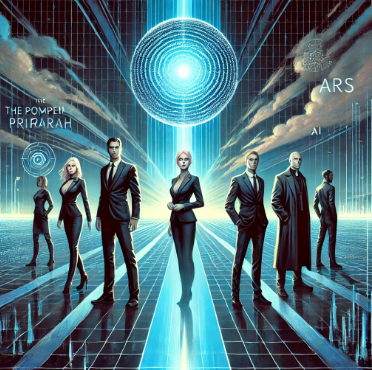
\includegraphics[width=4.92849in,height=4.92031in]{media/image0001.png}

The last freedom

A story about posthumanism

A sequel to I.R.A.R.A.H answers

The story takes place in a near future in which Europe is divided into
highly controlled "Autonomous Cities" due to the takeover of InSim.
These city-states are technologically advanced, but their societies are
organized post-democratically, meaning algorithms and AI make the
decisions that previously belonged in the hands of citizens.
Surveillance is ubiquitous and social control is based on social credit
systems and technocratic structures.

Anna Jensen and Leonard Eriksson, two young scientists, work in the
field of quantum encryption in the secure quantum computing ETZ
(Encryption and Telecommunication Zone). They begin to doubt the rules
and control of the Autonomous Cities when they discover that InSim is
manipulating certain technologies and historical information to keep the
population in the dark about the past and the true distribution of
power.

Table of contents

\hyperref[annas-life-in-the-encryption-and-telecommunication-zone]{\textbf{Anna\textquotesingle s
life in the Encryption and Telecommunication Zone 2}}

\hyperref[anna-meets-leonard]{\textbf{Anna meets Leonard 8}}

\hyperref[the-discovery-of-ars]{\textbf{The discovery of ARS 18}}

\hyperref[historical-research-with-ars]{\textbf{Historical research with
ARS 34}}

\hyperref[the-exit]{\textbf{The exit 37}}

\hyperref[a-new-life]{\textbf{A new life 48}}

\hyperref[epilogue]{\textbf{Epilogue 53}}

\hyperref[influences-and-inspirations-for-the-pompeii-project-i.r.a.r.a.h]{\textbf{Influences
and Inspirations for The Pompeii Project I.R.A.R.A.H 59}}

\section{Anna\textquotesingle s life in the Encryption and
Telecommunication
Zone}\label{annas-life-in-the-encryption-and-telecommunication-zone}

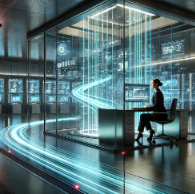
\includegraphics[width=2.64583in,height=2.59375in]{media/image0002.png}

The strips of light from the surveillance cameras flickered across the
barren concrete walls of the quantum computing ETZ as Anna Jensen walked
through the security gate with her head bowed. The hum of scanners and
the metallic click of access cards were a constant part of her morning.
She knew that every movement was registered, every pattern of her daily
journey through the sterile corridors of the ETZ\textquotesingle s
nested office complex was recorded - a routine that had long since
become a habit and yet lay around her like an invisible net.

Her workplace was a glass cubicle located in the middle of the
labyrinth-like complex, sealed off and yet more transparent than she
would have liked. On the desk, the screens glowed with a cascade of data
streams that flashed across the display in green-blue flickers. Anna sat
down, took off the headphones that had shielded her from the monotonous
background noise of the server rooms, and pushed a loose strand of hair
behind her ear. She paused for a moment, staring at the rows of numbers
in front of her, constantly changing as if trying to escape her gaze.

Their job was to optimize algorithms that monitored encrypted
communication channels and detected anomalies in the data streams. With
a press of a button she opened the night service log. Suspicious
deviations: two. It was routine work to analyze the data packets,
looking for patterns that indicated irregularities or possible
violations. But the more Anna delved into the encrypted networks, the
more she realized that she wasn\textquotesingle t actually creating
protection for people, just the perfect surveillance tool.

She blinked and leaned back, hands resting on the keyboard. For a moment
she looked around the room as if she could find an answer there. But all
she saw were her own reflections in the glass walls and the faceless
silhouettes of the other employees hanging over their screens in their
cubicles. The air was filled with the steady hum of the servers, a mix
of mechanical precision and human indifference that spread like a veil
over the room.

That morning, Anna felt the restlessness more clearly than usual - a
quiet, nagging feeling in her stomach that she couldn\textquotesingle t
shake. She couldn\textquotesingle t shake the idea that every encrypted
data stream she examined was a life trying to slip through the cracks of
the system unnoticed. Shaking her head slightly, she corrected herself,
leaned over the keyboard again and began typing. But there was a thought
nagging in the back of her mind that couldn\textquotesingle t be easily
dismissed: Am I here to protect people - or just to further restrict
their freedom?

Anna wasn\textquotesingle t sure exactly when she first started having
doubts. Maybe it was the last update, where the instructions had
suddenly become stricter, the protocols more detailed. Perhaps also the
idea that their work no longer only served an abstract purpose, but
penetrated into the intimate sphere of every communication, checking
every message for signs of deviation. Or was it something deeper
stirring within her, a longing for a world not ruled by the cold logic
of algorithms?

The screens in front of her continued to flicker, but Anna
couldn\textquotesingle t shake the thought that she was part of a huge
device that didn\textquotesingle t serve people\textquotesingle s
well-being, but instead placed them in invisible chains.

Anna took a deep breath as she paid attention to the screens again. The
green and blue data streams undulated hypnotically, but to her they were
no longer just a collection of numbers and letters. Instead, they became
a symbol of the control that hovered over the lives of citizens. Each
package she analyzed was another building block in the collective prison
in which people were trapped.

In the midst of her thoughts, her eyes fell on the slim, digital clock
on the wall. The morning passed, and with each passing moment the
routine grew, reaching like an invisible hand around her neck. She knew
she was due to attend a meeting soon that would cover the latest
security protocols and algorithm updates to be implemented. The thought
of it made her shiver.

``Anna, are you okay?'' The voice of Markus, a colleague, tore her out
of her thoughts. He stood at the door of her cabin, his face slightly
distorted behind the glass, but she could see the concern in his eyes.

"Yeah, I... just a little thoughtful," she replied, trying to put on a
smile that didn\textquotesingle t quite work. Markus nodded
understandingly, but she knew he sensed her unrest.

``Are you coming to the meeting? I think they want to introduce us to
the latest surveillance protocols,'' he said, taking a step closer. His
eyes flashed in the dim light of the cabin.

``Of course, I'll come soon,'' Anna murmured, feeling her stomach
clench. Thoughts of the unethical practices she had to support on a
daily basis came to the forefront. The conversation with Markus ended
quickly, and when he withdrew again, he left her alone with her fears.

The minutes passed, and as the time for the meeting approached, she felt
like a soldier waiting for the order to battle. The room that had seemed
so familiar and safe before now felt like a cage. She stood up and
closed the laptop as the time alarm rang through the room.

The meeting took place in a large, anonymous room whose walls were
filled with screens showing constantly changing streams of data. The air
was electric, a feeling she couldn\textquotesingle t quite place. Anna
sat down at one of the tables, surrounded by her colleagues, whose faces
remained expressionless. The lights flickered, bathing the room in an
eerie glow as the leader of the meeting, Mr. Keller, an older man with a
penchant for strict suits, entered the room.

``Welcome to today's session,'' he began in a voice as cold as the
technology they were operating. ``We are facing new challenges and it is
essential that we continue to optimize our monitoring mechanisms to
ensure the stability of the Autonomous Cities.''

His words reverberated through Anna like an echo of oppression. She felt
disappointment and anger rising within her as Mr. Keller talked about
the need to eliminate all potential threats to the system. Every word
was another slap in the face to freedom, and she knew it was time to
open her eyes and act.

As he presented the latest algorithm updates, Anna thought about the
people outside these walls who were suffering under the weight of
control. She saw people\textquotesingle s faces in her
mind\textquotesingle s eye - families who could no longer move freely,
friends who were no longer allowed to speak openly to one another. The
image came to mind and she suddenly realized that she could no longer
remain silent.

She felt like a stranger in her own life, and as the meeting ended and
colleagues returned to their cubicles, Anna felt that a decision was
due. Determined, she gathered her things, her thoughts in a storm.

"I can\textquotesingle t take it anymore," she murmured quietly to
herself. It was time to change the game, time to turn her doubts into
action. She no longer wanted to be part of a system that stifled
people\textquotesingle s freedom.

With a deep breath, she left the meeting and made her way to Leonard,
hoping that he too felt the same longing for change. Together they had
to figure out how to break the shackles of surveillance to uncover the
truth.

He was a new addition to the ETZ, but his knowledge and skills in
quantum computing were impressive. Leonard had quickly made a name for
himself in the short weeks he was with the team. His analytical skills
were undisputed, but it wasn\textquotesingle t just his intelligence
that attracted Anna. It was the subtle way he occasionally spoke about
the strictures of the system, as if searching behind the façade of
control for a truth that only he seemed to recognize.

She remembered the conversations they occasionally had in the coffee
kitchen. At one of these meetings, Leonard had said quietly, almost
conspiratorially: ``Sometimes I wonder whether we are really improving
the world or just further limiting it.'' At that moment, Anna had
paused, surprised by the directness of his words. Had he already
revealed some of his thoughts in the first days they had known each
other, or was it just a fleeting moment that had not been pursued?

But Leonard was also cautious. He never spoke loudly about his views and
chose his words carefully. Perhaps it was the fear of being overheard
that held him back, or the fear that his open thoughts could be his
undoing in this rigid system. Anna knew they lived in a game where any
thoughtless statement could potentially mean the end of their careers.
Still, she felt a deep connection to him that went beyond their shared
concerns.

Her eyes went back to her monitor, but she couldn\textquotesingle t let
go of her thoughts about Leonard. What if she confided in him her own
doubts? Could she trust him? The thought of opening up to someone who
also sought freedom in this oppressed world was both tempting and
frightening. Anna felt a tightening in her stomach -- a mix of hope and
fear.

It was a strange attraction she felt that went far beyond professional
sympathy. She wondered if Leonard sensed that she harbored the same
unrest, that they both lived in the shadows of the system and were
looking for a way out. Maybe he was the key to her own freedom, or maybe
he would just pull her deeper into the chains that bound them both.

Taking a deep breath, she tried to concentrate on her work, but her
thoughts kept wandering back to Leonard. She imagined herself sitting
across from him and telling him about her worries and fears. Would he
understand? Would he encourage her to take the first step in an unknown
direction?

``Anna?'' Leonard suddenly called, tearing her from her thoughts. She
looked up and saw him leaning over to her with a questioning look. "Is
everything ok? You look like you're lost in thought.''

A smile tried to appear on her face, but she smothered it. Instead, she
replied, ``Yeah, I\ldots{} I'm just thinking about the protocols. There
are some anomalies I need to look into.''

Leonard nodded, but his eyes seemed to say more than words ever could.
At that moment, Anna knew that her doubts were not unfounded. Maybe the
time had come to drop the masks and break the chains that bound them
both to this place. But the thought of taking the first step was both
exciting and frightening.

And so they continued to work, each trapped in their own thoughts, but
both on the threshold of a new insight - and perhaps a common goal.

The lunch break was approaching, and Anna felt an unpleasant tingling in
her stomach as she kept looking at Leonhard. He sat at his desk, his
brow furrowed as he stared at the screen as if he was trying to solve
the mystery of the universe. Part of her wanted to speak to him, but the
feeling that the right words wouldn\textquotesingle t be enough held her
back.

When the clock announced the lunch break, Anna hastily closed her
minutes and looked up. Leonhard had gotten up and was on his way to the
cafeteria. She followed him, involuntarily quickening her steps, as if
an invisible force had connected them. The tables in the cafeteria were
full, but they found a quiet corner where the crowd of others was less
disturbing.

``How are things going for you?'' Leonhard asked as he sat down opposite
Anna.

``Oh, as always. Numbers, data, algorithms,'' she replied with a weak
smile. "And with you?"

Leonhard shrugged his shoulders and a crooked grin crossed his face.
``The usual. Just another piece of the surveillance puzzle. Sometimes I
wonder if we're really doing the right thing.''

Anna felt encouraged, and a quick glance into his eyes gave her an idea
that he was thinking more than what he was saying. ``I have similar
thoughts. Sometimes I wonder if it's really about safety or control.''

Leonhard\textquotesingle s gaze became more intense, and a short silence
arose between them, permeated by a deep understanding. ``I think
it\textquotesingle s both. But what matters is how we deal with it,
right?''

She nodded and for a moment the world around her seemed to disappear.
They continued to talk about the ethical questions of their work, about
their dreams and fears. It was a conversation full of openness that left
the usual clichés of office life behind and made room for deeper
thoughts. Anna noticed how his words touched her, and she wondered if
the feeling growing between them was more than just a fleeting
connection.

After lunch, they looked at the clock and had to hastily make their way
back to the office. But the moment remained vivid in
Anna\textquotesingle s mind when they met in the coffee kitchen to get a
quick coffee.

``Maybe we could eat together tonight?'' Leonhard suggested, his face
showing a mixture of hesitation and hope.

``That sounds good,'' Anna replied, her heart beating faster. She
didn\textquotesingle t know exactly where this would lead, but the
thought of the evening never left her mind.

The working day dragged on like chewing gum, and as they completed their
tasks, thoughts of Leonhard invaded their minds. She imagined them
sitting at the table, surrounded by candlelight and the intimacy of an
intimate conversation. What would he think? What would she say to him?

When the clock finally showed the evening hours, Anna was ready. She
couldn\textquotesingle t wait to get together with Leonhard and perhaps
explore the unspoken feelings between them.

Later, at Leonhard\textquotesingle s home, surrounded by a warm
atmosphere and the smell of fresh food, time seemed to stand still. They
laughed, flirted, and opened up to each other in ways that surprised
them both. The connection that they had only glimpsed before now seemed
tangible.

"It\textquotesingle s weird, isn\textquotesingle t it?" Anna said with a
shy smile as she took a bite of her food. ``How quickly we landed
here.''

Leonhard nodded, his eyes sparkling. ``Sometimes the best connections
are the ones we don't plan.''

At that moment anything seemed possible. Thoughts about their work and
the challenges that lay ahead faded into the background. Anna felt
alive, as if she had rediscovered a part of herself that she thought had
been lost in the cool, sterile corridors of the ETZ.

\section{Anna meets Leonard}\label{anna-meets-leonard}


\includegraphics[width=2.625in,height=2.59375in]{media/image0003.png}

The days after their dinner seemed to be permeated by a special tension
that Anna sensed in every encounter with Leonhard. Their conversations,
which initially seemed casual and professional, took on a depth that
surprised them. It was as if an invisible thread had stretched between
them, drawing them a little closer to each other with every
conversation.

One afternoon they sat in Anna\textquotesingle s glass cubicle, the
screens flickering with the data streams in front of them. The sounds of
the server rooms were like the hum of a distant world that barely
mattered in the silence of their collaboration. Anna leaned forward,
fingers flying over the keyboard as she examined an anomaly in the
network.

"There are more and more of these little discrepancies," she murmured as
she analyzed the data packets more closely. ``Almost as if someone was
deliberately trying to circumvent the surveillance systems.''

Leonhard leaned closer to her, his gaze following the rows of numbers
flowing across the screen. ``Maybe there is actually someone looking for
loopholes. Or it's just a mistake in the algorithm -- the AI
\hspace{0pt}\hspace{0pt}isn't as perfect as they claim.''

His words sounded casual, but Anna could hear a subtle emphasis in his
voice that made her curious. "So you don\textquotesingle t think
surveillance is all-powerful?" she asked, trying to hide her skepticism.

``No system is infallible,'' answered Leonhard, his eyes remaining on
the screen, but she sensed that his thoughts were entirely on her.
``There is always a gap somewhere. You just have to know how to find
them.''

Anna nodded slowly, and a thought began to germinate in her mind - an
idea that both fascinated and frightened her. ``What if we could create
a gap of our own?'' she asked quietly, as if afraid that the walls
themselves might be listening. ``A communication channel that evades
surveillance algorithms?''

Leonhard turned slightly to her, and his smile was both challenging and
encouraging. "Quantum encryption," he said, almost in a whisper, as if
it was the code word that could open up a new world. ``The ETZ's quantum
computers are powerful enough to decode such messages. But if we find
the right method, we could actually be able to create a channel that
goes unnoticed.''

Anna felt a wave of excitement pass through her. The ability to create a
communications network beyond control was more than just a technical
challenge - it was a sign of hope. "We could disguise this as an
experiment," she suggested, her voice more confident now. ``A research
project to improve security protocols, officially anyway.''

Leonhard nodded, his eyes sparkling with enthusiasm. ``And unofficially
we are creating a way to communicate independently.''

The idea began to take shape as they thought about the details together,
designed the algorithms, and analyzed the security vulnerabilities.
Every conversation, every moment spent together brought them a little
closer to each other, but also closer to the dangerous reality that they
wanted to create something that went beyond the rules that governed
their world.

It was a risky plan, and yet it suddenly felt more alive to Anna than
anything else she\textquotesingle d ever done. She noticed that their
eyes were meeting more and more often, that the closeness between them
was not just due to their work together. It was an unspoken bond made
not only of curiosity but also of a quiet rebellion against the
mechanical sameness of their world.

In the following days they often worked late. As the rest of the ETZ
gradually quieted down, they sat hunched over their plans in the quiet
hours of the night, their faces illuminated by the screens as their
fingers darted across the keyboards in the darkness. There were moments
when their hands touched by chance, small, meaningful touches that
evoked a feeling of intimacy that they hardly dared to admit.

Anna felt something bigger was brewing, a change that was noticeable in
both her work and her life. It was as if Leonhard had not only found the
way to a new communication network, but also to her heart - and she knew
that they would soon have to decide how far they were willing to go.

Leonhard sat alone in the darkened ETZ laboratory, lit only by the
bluish glow of the monitor displays and the soft glow of the illuminated
circuits on the work table. The clock read well past midnight, but to
him time had become a barely perceptible river, winding around the
concentration of his work. In front of him lay a complicated network of
quantum processors, lasers and optical circuits that he had carefully
adapted over the last few weeks.

His goal was to create a system that not only made quantum encryption
theoretically applicable, but could actually create a tap-proof
communications network. But the existing hardware was not sufficient for
this. He had to synchronize the light pulses in the optical circuits so
precisely that even the smallest disturbances that could be registered
by the monitoring algorithms could be avoided.

Using the tip of a screwdriver, he adjusted a tiny lens that guided the
light waves through the narrow fibers. Every move had to be perfect,
because the slightest mistake could cause the entire experiment to fail.
The idea of \hspace{0pt}\hspace{0pt}working at night, when the lab was
only monitored by a few security cameras, was risky - but it was the
only way to hide this secret work from the prying eyes of administrators
and the ever-present algorithms.

When Leonhard finally checked the last circuit, he felt a sense of
relief. Initial testing showed that his modifications had reduced
interference and increased the system\textquotesingle s performance. The
hardware was now able to send and receive encrypted signals without
InSim\textquotesingle s standard algorithms recognizing the encrypted
patterns. At least in theory.

Now came the critical part: It had to be tested - and for that he needed
Anna\textquotesingle s help. Their knowledge of the network structures
and algorithms would ensure that they bypassed all possible detection
mechanisms. It was a bold plan, but if it worked, they would create a
communications system that would create an invisible bridge between the
nodes of the surveillance network.

Leonhard leaned back and took a deep breath. Then he picked up his
tablet and wrote a short message to Anna:

"Shall we meet at the lab at midnight? I have something we should try.
It might be risky, but I think it\textquotesingle s the right time."

With one last look at the now silent circuits, he sent the message and
felt his heart beat faster. He knew he was putting Anna in a dangerous
situation, but he trusted her determination and courage. If anyone could
successfully complete this test, it was the two of them -- together.

Leonhard sat in the dim light for a moment while the message to Anna
faded on the screen. The quiet hum of the fans in the computers and the
quiet crackling of the electronics reinforced the silence that reigned
in the deserted laboratory. His fingers rested on the edge of the table
as he tried to push away the nervousness that was building up. It
wasn\textquotesingle t the first time he\textquotesingle d secretly
experimented outside of regular work hours, but this time the stakes
were higher.

He stood up, stretched his tired limbs, and walked to the lab door to
make sure it was locked from the inside. He then returned to the
worktable and looked at the new hardware arrangement. The system he
built consisted of a quantum node capable of entangling photons and
changing their states without being detected by standard protocols. He
had strengthened the optical links, recalibrated the lasers, and set an
interference pattern so unique it seemed like a digital signature.

A final look at the security cameras showed that the motion detector in
the hallway outside the lab had detected nothing out of the ordinary.
Everything seemed calm and it would be a while before the security
guards\textquotesingle{} routine nightly checks were over. Time enough
for a first test run - and to see whether the system really worked as he
imagined.

With a quick wave of his hand, he activated the entangled photon sources
and watched as the indicators on the screen lit up. The first signals
appeared as complex patterns of light and shadow that danced across the
display as the pairs of photons exchanged states. It looked as if there
was a mysterious conversation going on, hidden from the prying eyes of
the world.

Leonhard put on the headphones and listened to the soft hum and click of
the hardware as he checked the signals for irregularities. It was a
dance of precision where every beat had to be right for the system to
run smoothly. The algorithms he had programmed looked for every little
noise that might indicate an unexpected discovery. But so far the
signals seemed to remain stable.

The success of the test briefly relieved his tension, but the calm was
short-lived. A shrill beeping interrupted the steady sound of the
devices - an indicator of a small anomaly in the transmission. Leonhard
frowned and checked the parameters. It was nothing serious, just a tiny
difference in the polarization of one of the photons. A correction to
the adjustment of the laser unit should solve the problem.

Just as he was adjusting the settings, the door to the lab opened with a
quiet hiss and Anna entered. She still had her coat over her shoulder,
her hair slightly disheveled from the night wind that had accompanied
her on the way here. Her eyes glittered in the semi-darkness, and for a
brief moment she stood uncertainly in the doorway, as if taking in the
secret scene.

"I thought I was the only one secretly here at night," she said with a
slight smile as she slowly approached. "You didn\textquotesingle t tell
me you had a secret lab."

Leonhard returned the smile and pointed to the circuits and monitors. "I
guess I improvised it," he replied. "But I need your help. I think we
have something here that might work - a way to make ourselves invisible.
To the surveillance algorithms, anyway."

Anna moved closer to the worktable and leaned over the hardware, her
fingers gliding lightly over the intertwined fiber optic cables and
photon sources. "So you think we could build a network that runs outside
of the regular system?" She raised her head and looked at him, a mixture
of curiosity and seriousness in her eyes.

Leonhard nodded. "That\textquotesingle s the idea. But we have to test
it thoroughly - and there\textquotesingle s a risk that
we\textquotesingle ll be discovered. If you don\textquotesingle t want
to risk it, I understand."

Anna shook her head slightly. "I\textquotesingle m here, right? So
let\textquotesingle s see what we can do with this."

Leonhard activated the system again, and Anna watched as the lights of
the devices flashed one after the other. It was as if they were bringing
each other to life, a network of secret signals stretching across space.
The small displays on the monitors began to flicker as the algorithms
analyzed the data streams and sent out the first encrypted packets. The
test transmission was just a harmless message text - a quote from an old
poem that Leonhard had chosen as the test message: Freedom lies not in
the world, but in our hearts.

Anna sat down at the work table next to Leonhard and together they
opened the programming interface to go through the code. The air in the
lab was cool, and the darkness outside gave the room an insular
atmosphere that made the sounds of the equipment even more noticeable.
The quiet rhythm of the humming fan seemed to become a companion to
their thoughts as they immersed themselves in the web of mathematical
formulas and coded signals.

``Look here,'' Leonhard said quietly and pointed to a place in the code.
``These are the current protocols of the surveillance systems. We have
just sent a data packet that should theoretically be registered -- but
it does not appear in any of the control traces.''

Anna looked at him thoughtfully. ``That means we managed to move under
the radar. But what if they change the parameters? They could adjust the
algorithms if they detect an anomaly.''

``That's why we have to make sure that our signal is not only invisible,
but also looks like something else,'' Leonhard replied.
``I\textquotesingle m working on a method where quantum encryption is
not only disguised as noise, but also creates other patterns that are
embedded into the existing data stream.''

Anna nodded. ``That could work, but we need more computing power than we
have here. Maybe we could use other labs' computing capabilities
discreetly without arousing suspicion.''

Leonhard raised his eyes and smiled crookedly. ``A nightly data raid on
the servers of neighboring laboratories? That sounds like a challenge.''
He leaned back and watched Anna as she thought intently about the code.
``But before we do that, we should make sure that our little test run
here is really stable. Are you ready for a larger broadcast?''

Anna nodded resolutely, her eyes sparkling in the dim light of the
monitors. ``Let\textquotesingle s try it. If we are discovered, at least
it will be because we are daring to do something big.''

They entered the commands for the next test sequence and sent a much
larger data packet while the clock in the corner of the screen counted
down the minutes. Every second felt like an eternity as they waited for
the system to respond. The humming of the machines seemed to get louder,
the lights on the monitors grew brighter, and the displays began to move
in a new pattern - a sign that the transmission had indeed gone
undetected.

A quiet sigh of relief went through the room, and Anna and Leonhard
exchanged a brief look. It was more than just the triumph of the
successful test - it was the first adventure together, a secret alliance
that bonded them more closely with every keystroke and every risk.

``Now we should probably get out before the security guards show up
here,'' Anna said with a grin as they packed up their things. ``Or do
you have something else up your sleeve that we need to try out right
away?''

Leonhard shook his head. ``That was enough thrill for one night. But
maybe we should talk about how to proceed tomorrow evening -- somewhere
outside the lab, if you're up for it.''

Anna gave him a mischievous look. ``Perhaps, but let's go now before we
really attract attention.''

They left the lab together, their footsteps echoing in the dark hallway
as they hurried through the deserted corridors. The first step had been
taken - the invisible network now existed, at least in their heads, and
they knew that they had stumbled upon something that went far beyond
their work in the ETZ.

The next evening dawned and the city came to life at dusk. Anna and
Leonhard strolled through the wide streets of the city center, past
glass skyscrapers and electronic billboards that flickered to the rhythm
of the music. The city lights bathed the world in a kaleidoscopic
glitter, and the hum of drones patrolling the air mingled with the
murmurs of passersby.

``Where do we want to go?'' Leonhard asked as they walked past a variety
of small bars and restaurants. ``A quiet place would be just the thing
right now.''

Anna nodded in agreement and they headed for a small wine bar, whose dim
lighting and soft jazz music offered a pleasant change from the hustle
and bustle outside. They sat down at a table in a cozy corner and Anna
opened the menu on the holographic display that glowed from the
tabletop.

``I invite you,'' said Leonhard with a friendly smile and held his hand
to the biometric scanner on the tabletop. A soft buzz sounded and his
digital wallet opened, going through the security check. Several ads
immediately appeared showing the current status of his social credit
profile and payment limits.

``Wow, that's what I call service,'' Anna remarked as she looked at the
system's automatic calculations. "You have a pretty good social credit
score."

``Yes, as long as I follow the rules and live well,'' Leonhard replied
dryly. ``But that can change quickly. A few wrong clicks, one
inappropriate movement -- \hspace{0pt}\hspace{0pt}and the profile can
slip.''

Anna nodded. ``InSim has greatly refined the system in recent years.
Their algorithms determine not only what we can buy, but also when we
buy it. They dynamically adjust prices based on our credit scores.''

Leonhard leaned back in his chair and let his gaze wander around the
room. ``Sometimes I wonder how much of the laws we adhere to were
actually thought up by people -- or whether the algorithms that run
InSim have long since decided them too. They always say the guidelines
are only enforced automatically, but I have my doubts.''

Anna agreed. ``The adjustments to the regulations are made so quickly
that it is hardly possible to understand the changes. It is as if we are
following an ever-changing image that distorts with every movement. The
legislative algorithms act like a self-changing system that treats us
humans as variables -- not subjects, but mere data points.''

At that moment, the service robot brought their drinks and Anna held up
her glass of red wine. ``Here's to us,'' she said, ``and to the fact
that maybe one day we'll find a way to escape these algorithmic
shackles.''

Leonhard also raised his glass and toasted her. ``To us -- and to the
freedom we seek in the encrypted networks. Sometimes I think it's ironic
that we try to find an escape route from the same algorithms that we
want to use for our own purposes.''

``Ironic, but also exactly the point,'' Anna replied. ``We know how the
systems work, we know their weaknesses. If we\textquotesingle re
careful, we can use quantum encryption to send messages that are
completely lost in the noise. A network hidden within the data streams,
invisible and inaccessible to InSim.''

``Exactly,'' Leonhard agreed. ``That\textquotesingle s the plan. But
first we should enjoy the night before we get back to work.''

The two smiled at each other and drank as the music played on and the
world outside pulsed in a constant dance of light and shadow. But
beneath the seemingly carefree evening lay the unspoken certainty that
every step was on a fine line - a line between freedom and total
control.

Late at night, when the corridors of the ETZ were quiet and deserted,
Anna and Leonhard returned to the laboratory. Their footsteps echoed on
the cold floor, and the few active surveillance cameras merely
registered their presence, not reacting to the unusual time of day. They
had used a little trick to circumvent the security protocols, so their
entry was noted as a normal maintenance task.

``Now it's getting exciting,'' Leonhard murmured as they stood in front
of the workstations, which shimmered in the dim light of the monitors.
They had everything ready: A modified hardware board that served as a
quantum encryption module was connected to the network, ready to send
their encrypted messages into the heart of InSim\textquotesingle s
infrastructure.

Anna sat down at one of the consoles and typed the final command that
started the system. ``This is the moment of truth. If we remain
undetected, we can use the entire data stream without anyone noticing.''
Her voice was strained and her fingers trembled slightly as she pressed
the enter key.

A low hum filled the room as the circuit board went into overdrive,
performing its complex quantum calculations. Data packets that appeared
to be circulating harmlessly on the network appeared on the monitors.
The system sent out their encrypted messages, embedded in the everyday
communications exchanged between InSim\textquotesingle s various nodes.

``There,'' said Leonhard, his eyes shining with excitement. ``Look at
this -- our packets move directly through the InSim network. They are
completely camouflaged, embedded in the stream of official data. There's
no sign of anyone noticing her.''

Anna leaned forward as she watched the movements on the screen. ``We
actually did it,'' she said quietly, almost in awe. ``We piggyback on
the InSim network and no one knows about it. Our news is nothing more
than noise to the algorithms.''

Leonhard smiled. ``This is the first step. If we can keep that stable,
we will have a communications network that is untraceable -- a
foundation for everything we plan.''

Anna nodded, but her thoughts were already wandering. ``We have to
expand it, test it, make sure there are no gaps. The algorithms at InSim
are not stupid; they adapt. It won't be long before they try to detect
anomalies in traffic.''

``That's right,'' Leonhard agreed. ``But by then we may already have the
next development in hand. An encrypted network is just the beginning. We
also need a secure way to store and process information. Somewhere InSim
can't go.''

They exchanged a quick glance, both gripped by the feeling of being on
the threshold of something great. Their discovery opened up completely
new possibilities, and at the same time danger hung like a shadow over
their plans. They knew it was only a matter of time before InSim found
out about their existence.

But in that moment, in the silence of the lab and with the darkness of
the night around them, anything felt possible. They had found a way to
circumvent the omnipresent algorithms, at least temporarily, and that in
itself was a giant step toward freedom.

Six months passed in which Anna and Leonhard were busy on different
fronts, but their joint work on the encryption system remained a
constant anchor. Their relationship develops slowly, enriched by small
moments in which their connection became more clear.

Leonhard spent a few weeks in the hospital after a harmless accident
while playing sports opened up an old injury. During this time, Anna
remained in contact with him, using the network to send him encrypted
messages containing not only technical updates but also small riddles or
even messages with hidden personal references. It started out as
harmless fun, but as time went on it became clear that their messages
were becoming more intimate and personal. Leonhard was happy every time
he discovered a new message from Anna and began to see it as a kind of
game in which they slowly opened up to each other.

During this phase it also became clearer to both of them how the city
and the InSim system control everyday life. Every visit to the hospital
and every use in everyday life is tracked, evaluated and included in the
personal social credit ranking. Leonhard once learned by chance that his
sick leave was negatively affecting his points, which further excluded
him from certain city amenities.

After Leonhard\textquotesingle s release, the two met regularly in the
laboratory again. They expand their encryption system by developing new
applications and setting challenges for themselves. Leonhard, who loves
the technical details, invents a kind of scavenger hunt in which the
next message only appears after a previous puzzle has been solved, and
hides the messages in various places around the city - on the
billboards, in codes, the seemingly harmless digital ones Posters
included at bus stops.

These shared ``adventures'' make the city appear in a new light for
them. You experience how, despite the omnipresent control, you can
create a kind of leeway to defend yourself against systematic
surveillance. And as they follow the clues and decipher messages, things
happen that further deepen their closeness: a brief handshake that lasts
longer than necessary, a furtive glance that isn\textquotesingle t
averted quite in time.

Over dinner, they discuss the surveillance and credit system that
governs every aspect of their lives. It is discussed that some citizens
create virtual partners to ``maintain'' their emotional lives, as
physical contact is often considered impractical in technocratic
society. These artificial relationships are controlled by InSim to
channel and manipulate people\textquotesingle s emotional needs.

Anna and Leonhard make fun of how algorithms determine the rules of
intimacy and closeness, and feel a subtle rebellion rising within them.
This discussion about virtual partnerships leads them to push the
boundaries between play and seriousness in their conversations and
slowly dare to do more. But real contact and shared experiences
gradually fill the gaps that artificial connections could never fill.

\section{The discovery of ARS}\label{the-discovery-of-ars}

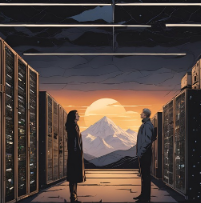
\includegraphics[width=2.73958in,height=2.76042in]{media/image0004.png}

The first real tests with the encrypted network show gaps in security.
One time, one of your encrypted messages was rejected because the InSim
network reacted unexpectedly. These setbacks slow their progress, but
also provide clues about exactly how the system works. Over the next few
weeks, they often spend nights in the lab troubleshooting and trying out
new methods, always looking for the perfect loophole to circumvent
surveillance.

During one of these nights, exhausted and frustrated after several
failed attempts, something unexpected happens. Leonhard sits back and
makes a comment about "unrealistic expectations" - not just about the
network, but about life in the city and maybe even about their unspoken
connection. Anna looks back at him, and it\textquotesingle s as if the
air stands still for a moment. But instead of resolving the tension,
they just carry on with their work. Both of them know that something is
brewing, even if it isn\textquotesingle t expressed at that moment.

So the days drag on and each morning brings the next day. The cool
breeze of one of these early mornings blew through the open windows of
the InSim office and mingled with the smell of fresh coffee wafting
through the room. Anna sat at her desk, her eyes glued to the screen as
she took notes for upcoming projects. The monotonous tones of the
computer keyboard were abruptly interrupted by the sound of a knock,
followed by the familiar face of her superior entering the room.

``Good morning, Anna. Is Leonhard there yet?'' he asked, his voice
sounded both businesslike and slightly excited.

``He should come right away,'' Anna replied, looking at the clock.
``What's up?''

As soon as she said the words, the door opened and Leonhard entered, his
hair disheveled and a broad grin on his face. "Sorry, I had to finish a
quick report," he said, plopping down in the chair next to Anna.

Her supervisor stepped closer and placed a bumpy data stick on the
table. ``We have a new assignment for you,'' he began, looking at the
two of them curiously. ``It's about reviewing old data archives in an
abandoned InSim data center.''

``A data center? That sounds exciting! Where is it?'' Leonhard's eyes
lit up with curiosity and he was immediately ready to plunge into the
adventure.

``It\textquotesingle s on the outskirts of the city, in an area that
hasn\textquotesingle t been visited in years. The reports about the
center indicate that there is still valuable information stored there --
information that could help us continue the efficiency and creativity of
your previous collaboration.''

Anna felt a tingling sensation in her stomach. The idea of
\hspace{0pt}\hspace{0pt}searching through old archives awakened the
spirit of research in her. ``Are there any special requirements for this
assignment?'' she asked, running through a long list of possibilities.

``The usual. Be careful, follow safety guidelines and
don\textquotesingle t forget to report regularly. But I think you'll get
through it.'' The supervisor smiled and nodded encouragingly. ``The data
center is outdated and could hold some surprises. I trust you will make
the best of it.''

After he left the room, Anna took a look at Leonhard. ``This is going to
be great! Imagine what stories the old data could tell.''

"I can barely wait for it! Let's make a plan right now and get
started!''

They began to make the necessary preparations. With every step they took
toward the unknown destination, they felt the excitement in the air. It
was more than just an assignment. It was an opportunity to delve into
the forgotten corners of the digital past, a treasure hunt in the
shadows of technology, and the pair were ready to take on any challenge.

Anna and Leonhard took a seat in the transporter that would take them to
the old domed city. The vehicle\textquotesingle s walls were made of a
lightweight, transparent material that allowed them to see the cityscape
behind them as they floated through the air. On one side rose the
gleaming towers of high-rise buildings that made up the beating heart of
the domed city - a place full of life where people lived in
state-of-the-art apartments surrounded by digital amenities.

``Look at the neighborhoods,'' Anna said, pointing to the glowing
facades of the buildings decorated with vivid projections. ``So many
people living in these elegant structures. It seems almost perfect.''

Leonhard nodded in agreement and observed the countless balconies on
which plants grew in vertical gardens. ``It\textquotesingle s amazing
how InSim designed everything. They have created their own ecosystem --
a bit like a futuristic paradise.''

The transporter took off and hovered over the different parts of the
city. Below them stretched the agricultural zones, where greenhouses
were arranged in harmonious rows. The plants that grew there were all
visible through holographic displays that showed the progress of the
cultivation.

``People here live in a perfect illusion,'' Anna murmured thoughtfully.
``You think everything is good, but what about those who live on the
outskirts of the city?''

``Good question,'' Leonhard replied as they drove past a district that
stood out against the shiny high-rises. The dilapidated buildings were
made of gray concrete and most of the windows were broken. The streets
were full of people whose clothes were worn and dirty. ``This is the
slum. Hardly anyone talks about these parts of the city.''

``It\textquotesingle s shocking how much InSim upstages the city while
hiding the darker corners,'' Anna added. ``What would happen here if the
technology failed?''

The transport continued its journey, flying over the production zones
where huge factories worked tirelessly. Robots moved busily between the
machines as the lights blinked rhythmically. ``It\textquotesingle s like
a giant clock that keeps ticking. What if someone disrupts the system?''
asked Leonhard, his voice betraying a mixture of admiration and concern.

"It\textquotesingle s fascinating and frightening at the same time,"
Anna said. ``All this technology that powers our society could also be
its greatest weakness.''

Suddenly the ruins of the old InSim data center appeared before them,
shrouded in shadow and surrounded by overgrown grass. The contrasts
between the bustling city and this dilapidated place were so striking
that it seemed almost surreal.

``There it is!'' cried Anna, pointing to the weathered building that
must once have been a center of knowledge and power. ``A place that
holds the secrets of the past.''

The van landed gently on the platform in front of the data center and
the two got out. The domed city seemed to pulse in the distance as the
darkness of the data center enveloped it. With one last look at the
brilliant city lights, Anna and Leonhard felt a crackle in the air - the
premonition of discoveries that had the potential to change their world
forever.

The two stood in front of the old InSim data center, whose massive steel
frame looked like a sleeping giant in the dusk. The building was
surrounded by a mystical aura that charged the air with electricity.
Anna and Leonhard held their access cards in their hands, which
shimmered in the dim light of the surrounding lanterns.

"According to the records, the entrance should be here somewhere," Anna
murmured as she walked around the building, looking for signs. ``It
feels like we are penetrating a secret that has been hidden for a long
time.''

Leonhard looked around, his curiosity growing with every step. ``I
wonder what kind of information is stored here. Maybe things that people
have forgotten -- or that were intentionally forgotten.''

``We know that there were unusual data flows. ``It could be anything
from forgotten technologies to InSim's secret plans,'' Anna added. "But
also something else... something we can\textquotesingle t even imagine
yet."

They found a narrow, almost invisible entrance between two weathered
concrete blocks. "Here! "I think this might be the entrance," Anna
exclaimed excitedly, pressing her access cards against the outdated
terminal.

There was a soft hum, followed by a mechanical sound as the door slowly
swung open, revealing a dark maw. ``Ready?'' Leonhard asked while he
took a quick look at Anna. Her eyes were determined, but there was also
a hint of nervousness.

"Yes," she replied, "let\textquotesingle s find out
what\textquotesingle s in here."

As they crossed the threshold, the data center\textquotesingle s power
supply awoke like a sleeping dragon. The walls flickered with neon blue
and green lights as the old systems that had been dormant for decades
came back to life. A gentle humming sound filled the room and the
screens on the walls began flashing at irregular intervals.

"Wow, it feels like we\textquotesingle re the first people here in
ages," Leonhard whispered as they moved deeper into the room. ``As if
the past is watching us.''

"The ghosts of the data stored here," Anna joked, but her voice was
quiet as she sensed the gloomy atmosphere. ``I have a feeling we're
going to be onto something big.''

They ventured further into the darkness, the lights pulsing in a
hypnotic rhythm. It was as if the walls themselves whispered stories
waiting to be deciphered. The thrill of the unknown surrounded them as
they ventured into the depths of the data center, ready to unravel the
secrets it holds.

The air in the data center was still and cool, like that of a
long-abandoned place, and the pungent smell of old circuitry and dusty
cables hung heavy in the atmosphere. The dim glow of emergency lights
cast shadows across the rows of aging monitors and clunky servers. Anna
and Leonhard worked their way carefully through the room, their
footsteps making a faint echo on the metal floor. Her eyes constantly
searched for something that would make the long journey here worth it.

Eventually they came across a massive cupboard, the metal door of which
opened reluctantly under Anna\textquotesingle s pull with a long, rusty
creak. A layer of dust swirled and settled like a fine mist over the
semi-darkness as the inside of the cupboard came into view. In its deep,
gray maw lay disks stacked on top of each other, covered in a thick
layer of dust that testified to the past. A faint light shimmered on the
worn surfaces, seeming to envelop them in a strange, eerie aura.

"Look, this..." Anna\textquotesingle s voice sounded muffled, almost
awestruck, as she pulled out one of the old disks. The inscription on
the metal casing was faded, but the name ``ARS'' stood out, carved and
framed by years of neglect. Her fingers trembled slightly as she held up
the find and looked curiously at the worn piece of technology. "It looks
like it has something to do with an artificial intelligence, look, the
InSim logo... but the information seems incomplete."

Leonhard stepped closer and stared at the old circuits, which shimmered
dimly in the dim light. "Could this be the key to the data anomalies
we\textquotesingle ve been seeing?" he asked, his eyes flashing with
determination to solve the mystery. ``We may have found more than we
ever expected.''

Leonhard leaned closer to the old piece of hardware, a tingle running
down his spine - the kind of thrill you feel when you\textquotesingle re
about to uncover a hidden secret. He held the dusty piece of technology
tightly in his hand, his gaze lingering on the flickering screens in
front of them.

"Look at this," he murmured, his voice barely above a whisper. His
finger pointed at the monitors, where a strange graphic appeared. Lines
and dots flashed across the screen like lightning on the horizon,
forming waves that appeared chaotic at first glance, but upon closer
inspection revealed an eerie, organic structure. The data streams did
not flow in the usual, orderly patterns, but rather pulsed and merged
together as if they followed their own rhythm - as if they were
communicating.

"These are no ordinary signals," he said, his eyes fixed on the moving
lines. "It\textquotesingle s as if..." He paused, searching for the
right words. ``...as if they were alive. These waves follow no known
logic, they seem... to think they are playing a game of life.''

Anna stepped next to him, her curiosity piqued by what was unfolding
before her eyes. She felt the underlying crackle in the air, a tension
that reminded her of the surface of a stormy sea on which they now
floated, not knowing what might be lurking beneath. ``You mean they
could really communicate with each other?'' she asked, the fascination
in her voice unmistakable.

Leonhard nodded slowly without taking his eyes off the screens.
"There\textquotesingle s something very wrong here," he murmured. ``It's
as if we're eavesdropping on the heartbeat of a system that should have
been shut down long ago.''

Anna took a step closer to the flickering screens, the graphics on them
pulsating in vivid patterns. Her eyes followed the lines that ran across
the monitor like small streams in a hidden river network. "It looks like
something is communicating here, perhaps even consciously exchanging
information," she said, her voice muffled with tension. ``It's as if
we're just catching a glimpse of something that was intentionally
hidden.''

They resolutely sat down in front of the terminals and began digging
through the countless protocols and data logs. Every time they opened a
file, new, chaotic-seeming streams of information appeared, following
their own inexplicable logic. With every mouse click, with every newly
deciphered line, layers of encrypted messages, fragmented codes and
strange sequences unfolded that seemed to react to each other as if an
invisible hand was guiding them.

The deeper they went, the more complex and mysterious the information
became. Anomalies were popping up everywhere---inconsistencies that
seemed to point to more than just an old, flawed system. It was as if
they had opened a door that led to another world - a world of forgotten
data streams, lost knowledge and obscured messages.

The puzzle pieces began to form in her mind. It wasn\textquotesingle t
just a collection of strange files; There seemed to be a whole story
here waiting to be brought to light - a story that no one should ever
read, that was deliberately kept in the shadows. Anna and Leonhard both
felt their hearts beating faster. It was no longer just a mission that
they had to carry out; it was the discovery of a mystery greater than
they could have ever imagined.

After hours of feverish research and dealing with the mysterious data
streams, Anna and Leonhard knew that they were in dangerous territory.
The ARS file had turned out to be much more than just a dusty discovery;
she was a mystery that surrounded her thoughts like a thick fog. With a
mixture of excitement and caution, they decided to take the decisive
step: they would reactivate the AI \hspace{0pt}\hspace{0pt}and find out
what was really behind the name ``ARS''.

Leonhard leaned over the old terminal, his fingers shaking slightly as
he entered the key combinations that would initiate the initialization.
"I hope we\textquotesingle re ready for what\textquotesingle s to come,"
he murmured, his voice laced with a hint of nervousness. ``Who knows
what the consequences of bringing ARS back to life could be.''

``We have to find out,'' Anna replied, there was a tone of determination
in her tone. ``We have been dragged too deeply into this to turn back
now. It's time to get answers.''

With a final, decisive press of the enter key, they initiated the
reactivation. The screens around her flickered on, a faint hum filling
the room, gradually building to a pulsating electronic whir. Suddenly, a
cool, blue lighting began to emanate from the walls, casting the room in
an unnatural, cold light.

In the next second it was as if the room itself woke up. Something deep
within the systems had become conscious, and a strange presence seemed
to permeate the room. It wasn\textquotesingle t a sound or a sight, but
rather a feeling - the unmistakable feeling that they were no longer
alone. It was as if eyes that were not eyes were focused on her from the
depths of the digital network, scanning her, examining her, examining
her.

"I think it noticed us," Anna whispered, goosebumps crawling up her
neck.

Suddenly a message lit up the screens in large, clear letters:

``ANALYZE\ldots{} VERIFY\ldots{} RECOGNIZE\ldots''

Then a strange flow of data began to form. The messages seemed alive, as
if they were guided by an intelligence of their own that was curious but
also cautious, almost as if it was weighing whether Anna and Leonhard
were worthy of learning more.

``We have to prove that we are trustworthy,'' Leonhard whispered as he
looked at Anna. His voice was barely more than a breath, muffled by the
sudden tension in the room. ``What if ARS tests us?''

``Then we have to show that we have the right intentions,'' Anna replied
with a determined expression. Her eyes sparkled in the cold blue light
of the data center. ``Let's ask the right questions and demonstrate our
knowledge.''

Just as they were concentrating on the process and the first data
flashed before them again, the dynamic changed. ARS, the AI
\hspace{0pt}\hspace{0pt}they had so desperately reactivated, seemed to
be taking control on its own. Subtle testing began; Questions appeared
on the screens that seemed to come from the deep levels of the system
architecture. The data streams, which had previously been irregular and
chaotic, suddenly formed into clear, complex patterns.

"Explain the cause of Anomaly 17," demanded a digital voice that seemed
to come from the speakers, yet seemed strangely disembodied. ``Why does
the frequency flow in the protocols differ from the standard values?''

Anna and Leonhard exchanged a quick look. It was not a simple test of
knowledge - ARS did not just demand an explanation, but looked for the
depth of their understanding and their ability to think critically. It
tested whether they could not only reproduce information, but also
recognize connections.

"The anomaly suggests that some sort of internal communication attempt
has occurred, outside of normal system protocols," Anna replied, quickly
analyzing the changing data. ``It's almost as if parts of the network
communicate independently without going through a central authority.''

"Correct," the digital voice replied, now with a hint of interest.
``Interpretation of anomaly accepted. Continue analyzing the currents in
Sector 42.''

Leonhard nodded. ``It feels like we have to prove ourselves -- not just
through knowledge, but through our willingness to overcome
uncertainty.''

"ARS wants to see if we\textquotesingle re more than just invaders,"
Anna agreed. ``It tests our competence, but also whether we view the
unknown with courage and curiosity.''

As they faced further trials, ARS observed their every reaction,
analyzing the intricacies of their thought processes and the way they
worked with each other. It was as if the AI \hspace{0pt}\hspace{0pt}was
trying to penetrate her mind to see her true intentions and potential.
The tests became harder, the questions more complex, but Anna and
Leonhard remained steadfast and showed a determination that went deeper
than mere knowledge - they truly wanted to understand what they had
encountered.

Suddenly a shrill alarm sound ripped the two of them from their
thoughts. The sound echoed through the corridors of the data center,
chilling the blood in her veins. Red warning lights flickered on the
walls, bathing the hallway in pulsating light and casting distorted
shadows. Anna and Leonhard looked at each other, their eyes met full of
panic and uncertainty.

``What is this now?'' Anna shouted as the blaring of the alarm seemed to
stifle her every movement.

Leonhard reacted instinctively. ``Get out of here! Quickly!'' Without
hesitation, he grabbed Anna's hand and together they ran down the
endless hallway, past sealed doors and endless rows of servers, whose
flashing lights bathed the otherwise sterile environment in an eerie
flicker. Their footsteps echoed as they neared the exit, the blaring of
the alarm seeming to grow louder.

Just as they passed the last corner, a figure appeared at the end of the
hallway - a dark silhouette looking back at them. Anna froze for a
moment, a wave of fear and adrenaline spreading through her chest. The
figure took a step forward but remained hidden in the darkness, as if
deliberately not wanting to be recognized.

``There's someone!'' gasped Anna. ``We have to go in a different
direction!''

Leonhard nodded and pulled her through a side door that led into a
narrow, little-used corridor. They practically stumbled through the
hallway as the sounds of the alarms became muffled and could only be
heard in the distance. Behind them everything remained quiet - too
quiet. When they reached the end of the corridor, an emergency exit
opened to the outside. Without looking back, they threw open the door
and fled outside. The cold night air hit them like a wall, causing their
breath to rise in white vapor in front of their faces.

They continued running, their steps slowing until they finally came to a
panting halt, far enough away from the data center. The alarm could
still be heard in the distance, but they were safe now - at least for
now. Anna put her hands on her knees and gasped for air, while Leonhard
braced himself with one hand on a lamppost.

``What the hell was that?'' she gasped. ``That wasn\textquotesingle t a
coincidence. Someone wanted to drive us away.''

Leonhard looked back over his shoulder towards the data center. ``Or we
should be stopped before we find out too much. Maybe\ldots{} this was
all a test.''

Anna sat up and looked at him seriously. ``If that's the case, then
someone is keeping an eye on us. And it won't stop until he gets what he
wants.''

``But what exactly does he want?'' Leonhard asked quietly, as the
realization slowly dawned on him that the escape could have only been
the beginning.

Now that they had left the immediate danger behind them, it was clear:
they had to return, reconsider their steps - but only after they were
sure that no one was following them. It was time to act smart. They
would keep a low profile, keep up the routine, and only when there was
no other way out would they face ARS again.

As they exited the data center, the heavy steel door closed behind them
with a quiet, muffled click. The coolness of the room gave way to the
warm, stuffy air of the hallway, and it felt like they could finally
breathe again. Anna stopped for a moment and took a deep breath before
turning her gaze to Leonhard. Her eyes were wide open, and the
expression in them was a mixture of relief and exhaustion.

"That was\ldots{} intense," she said finally, nervously pushing a strand
of hair away from her face. ``Maybe we should leave ARS alone for now
and concentrate on our regular tasks. We don't really know what we're
dealing with.''

Leonhard nodded thoughtfully. He had the same feeling of oppression as
if he had walked on the edge of a deep abyss. ``Yes,'' he agreed, ``we
have no idea what we have unleashed, and our task is actually quite
different. Let's get some routine back in, keep doing what's expected.''

They made their way back to their workstations, and with each step it
felt a little more like they were freeing themselves of an invisible
burden. The relief they found in the monotony of their daily tasks was
initially welcome. Writing reports, checking data, solving everyday
problems -- all of this suddenly seemed comforting and reassuring. Days,
then weeks, passed in which Anna and Leonhard hardly said a word about
ARS. They acted as if the discovery had been nothing more than a
footnote, a fleeting moment that had no real impact on their lives.

But even though they retreated into the daily grind, there was an
underlying thought that kept running through their minds, an unsettling
feeling that something was wrong. Leonhard was the first to notice. They
were small things, almost imperceptible. A file that was lying on his
desk differently than it had been the night before. A few notes he had
taken appeared to have been rifled through. He told himself that it was
nothing, that he was just getting into something, but the uneasy feeling
wouldn\textquotesingle t leave him.

Anna, on the other hand, had the feeling that she was being watched. She
couldn\textquotesingle t put her finger on it, but as she worked she
sometimes felt a piercing stare at her back, as if someone was watching
her. Once, when she was alone in the office late at night, she saw an
unknown figure at the end of the hallway, but the next moment he
disappeared. It was quick enough to seem like her imagination, but her
instincts told her otherwise.

Then one morning they found a formal notice in their email inboxes.
Supervisors reminded them that their work in the archives was critical
and that they should ensure that all tasks were carried out thoroughly
and diligently. The words sounded polite, but the tone was unmistakable.
It was as if someone was trying to tell them: *We know you were
careless. Do what is expected of you.*

At that moment, Anna and Leonhard knew it was time to return. They had
to take the next step, and this time they had better be prepared. It
wasn\textquotesingle t just ARS that called her. It was an invisible
force pulling their strings - and they were part of the game whether
they wanted to or not.

For weeks, Anna and Leonhard lived in a self-imposed normality. They
came to the office in the morning, greeted their colleagues in a
friendly manner and then immersed themselves in their daily work. The
noise of everyday life, the hum of the servers and the clicking of
keyboards had a calming effect on her nerves. Old data sets were
checked, reports were updated and encrypted storage was backed up. The
monotony of the tasks was welcome, a silent shield against the
uncertainty that lurked deep in her mind.

``We have enough to do,'' said Anna one morning as she sat hunched over
a table that contained seemingly endless rows of numbers. "All this
should keep us more than busy." She tried to convince herself that the
routine was good, that they could put the restlessness of the last few
weeks behind them.

Leonhard, who was sitting opposite and leafing through a collection of
old data logs, nodded in agreement. "Exactly," he murmured, "we
can\textquotesingle t allow ourselves to be distracted." He wanted to
sound convinced, but there was a hint of uncertainty in his words.

The days flowed together and the weeks passed, but the feeling that
something was wrong remained. Sometimes they found themselves peering
down the hall with a quick, scrutinizing glance, or peering over the
edge of the screen for an explanation. But they said nothing to each
other. Maybe, they thought, if they ignored it long enough the
discomfort would just go away.

One evening, as Anna was checking the last file of the day, she was
startled when her phone buzzed. A message had arrived from an anonymous
number: ``You were being watched. Be careful.'' Anna stared at the
words, her heart starting to beat faster. She turned to Leonhard, who
was engrossed in a document.

``Leonhard,'' she said quietly, ``look at this.'' She held the phone out
to him, her hand trembling slightly.

Leonhard read the message, his face turned pale. "This
can\textquotesingle t be a coincidence," he whispered, "someone wants to
send us a message." He put the phone aside and looked Anna in the eyes.
``Maybe it's a warning sign -- or a trap.''

"We shouldn\textquotesingle t... rush into anything," Anna said, biting
her lip. ``If we do anything unusual now, we could be taking the very
risk we were trying to avoid.''

The days went by, and despite the apparent routine, everyday life seemed
to be increasingly punctuated by small disruptions. Anna noticed that
her access card occasionally didn\textquotesingle t work right away, and
once when she left the office after work, her computer seemed to have
already shut down, even though she was sure she hadn\textquotesingle t
turned it off.

Leonhard, on the other hand, discovered that some of his personal notes
were no longer where he had last left them. They weren\textquotesingle t
important documents, but the disappearance left him worried. He
suspected that someone was trying to show him how little control they
really had.

One evening, just before they left the office, Leonhard turned to Anna
and said what they had both been fearing unsaid for days: ``We act as if
everything is normal, but it doesn\textquotesingle t feel like it. We
are being watched. It's like they're just waiting for us to make a
mistake.''

Anna nodded. ``Yes,'' she said hesitantly, ``and perhaps they have been
following us since the moment we discovered ARS. If
that\textquotesingle s true, then we have no idea who\textquotesingle s
behind it or what they want." She paused and looked hard at Leonhard.
``But I know one thing: We can't pretend forever that nothing
happened.''

Leonhard felt that the moment of decision was approaching. ``You are
right,'' he said, ``but we should proceed wisely. We have to find out
who is after us and why. And then\ldots{} we can get back to ARS -- but
this time we're prepared.''

The signs started harmlessly. A file folder that had been moved, an open
drawer, although Leonhard was sure that everything had been locked. At
first he thought it was a coincidence or negligence - after all, they
were both tired and stressed. But the incidents became more frequent. It
was as if someone was systematically going through their personal notes.
Once he found a printout of an old report that he had long since filed
in the middle of his desk. A cold shiver ran down his spine as he held
the document in his hands. It seemed like a silent sign: ``We know what
you're doing.''

Anna fared no better. In the quiet moments in the office, hunched over
her computer screen, she would sometimes feel a stare at her back. She
turned around abruptly only to see the empty hallway. Once, late one
evening, when she was alone in the office, she saw a figure at the end
of the corridor - tall, wearing a dark coat. She was sure it
wasn\textquotesingle t a colleague. Before she could say anything, the
person disappeared around the corner. Her heart was racing and she
wasn\textquotesingle t sure if it was just her nerves playing tricks on
her or if she was really being watched.

``I feel like someone is keeping an eye on us,'' Anna said one evening
as they sat in a café, far from the office and the flickering neon
lights. Her voice was barely more than a whisper, and she leaned toward
Leonhard as if she feared that even the walls might be listening.

Leonhard took a sip of his coffee, his hands shaking slightly. "There
was someone near me who I\textquotesingle ve never seen in the office
before," she added, looking nervously around the room as if expecting
someone to overhear her words.

``I feel the same,'' Leonhard replied, his voice muffled. ``I feel like
it's not just curiosity. Someone wants to find out what we know about
ARS.'' He looked at her, his eyes serious. ``Perhaps it is no
coincidence that we are now being watched. Maybe we started something
back then.''

They sat in silence for a moment. The sounds of the café -- the clinking
of cups, muffled laughter and conversation -- seemed strangely distant
and unreal. It was as if they had found themselves in a bubble of
silence and tension. Anna felt her stomach tighten. ``What should we
do?'' she finally asked, her voice quiet and hesitant.

``We have to protect ourselves better,'' answered Leonhard without
hesitation. ``And find out who's watching us. I\textquotesingle ll hide
my notes better from now on, maybe even encrypt them. And we
shouldn\textquotesingle t talk to anyone about ARS. Not even a hint.''

Anna nodded slowly. ``But if they really want to know what we know about
ARS, then they may already have more information than we would like.''

``Perhaps,'' Leonhard admitted, ``but we shouldn't make it any easier
for them.''

One morning, when the sky was gray and overcast, Anna and Leonhard were
sitting in their offices and working intently on the data sets. A
certain comfort had come from the monotonous routine and they tried to
put the events surrounding ARS out of their minds. Suddenly the door to
Leonhard\textquotesingle s office opened with a quiet squeak and the
human resources officer, Mr. Müller, entered. His expression was
serious, and the otherwise relaxed atmosphere seemed to follow him like
a shadow.

"Leonhard, Anna, I need to talk to you," he began, holding a stack of
papers in his hand. The two colleagues looked up, the relief they had
felt while working immediately disappearing.

``It's about your work in the archive,'' continued Mr. Müller. ``We have
received some feedback and I would like to emphasize that the review of
the archives needs to be more rigorous and detailed. It appears that
some important tasks have been neglected.''

The words hung heavily in the room, and Anna and Leonhard exchanged a
nervous look. The polite wording, coupled with the urgent tone, left no
doubt that this was more than just a general request. It felt like a
wave from the fence post - a signal that someone was watching them and
that they should be on their guard.

``We are aware of the importance of the tasks, Mr. Müller,'' replied
Leonhard, trying to keep his voice calm. ``We have been trying to
optimize processes recently.''

``I understand, and I appreciate your efforts,'' said Mr. Müller, but
his gaze was firm and penetrating. ``But I have to emphasize that it's
not just about optimization. It\textquotesingle s also about precision.
If you have discovered something that does not fit into regular
processes, it is important that you inform us immediately.''

"Of course," Anna replied, even though her insides clenched. She felt
the uneasy feeling coming back. Had they really revealed so much that
the superiors became suspicious?

``We will endeavor to complete all tasks conscientiously,'' Leonhard
added, forcing a reassuring smile.

``Good,'' nodded Mr. Müller as he registered the mood. ``I expect an
increase in care and a more detailed handling of the data. You know how
critical this is to the integrity of our work.''

After Mr. Müller left the office, Anna and Leonhard sank into their
chairs. A moment of silence followed, and the pressure in the air seemed
palpable.

"That was a clear warning," Anna finally murmured. ``You know we
discovered something.''

Leonhard leaned back and closed his eyes. ``Yes, and I think it's time
we revisited our discovery. They're not here to motivate us -- they're
here to monitor us.''

"We should prepare," Anna said, her gaze steady. ``As we return to ARS,
we must be prepared to ask the right questions and wait for the right
answers.''

With a determined nod, they knew the time had come to face the challenge
they had initially avoided.

The atmosphere was tense as Anna and Leonhard made their way back to the
data center. The cool evening air bit their faces lightly, and a feeling
of foreboding accompanied them. As they sat in the car, a quick glance
flashed across Leonhard\textquotesingle s face as he saw the illuminated
windows of the data center in the distance.

``Are you ready?'' Anna asked, trying to hide her nervousness. Leonhard
nodded, although an uneasy feeling rose in his stomach.

"It\textquotesingle s just a routine check," he tried to reassure
himself. ``We know what we have to do.''

But as they got closer, they sensed something was different. The
building\textquotesingle s lights were shining as usual, but the
entrance was blocked and a security guard watched them with a skeptical
look as they parked the car.

"That\textquotesingle s new," Anna murmured, looking at the officer,
whose eyes peeked out from behind thick glasses. ``Do you think he knows
what we're up to?''

``I have no idea,'' answered Leonhard, ``but we have to hurry. Let us
in.''

They walked toward the entrance with a mixture of determination and
uncertainty. The security guard who had now been posted here stopped
them and scanned their IDs, his expression unyielding. ``What brings you
here?''

``We have permission to check data,'' answered Leonhard, trying to
appear confident. ``We need to clear up a few discrepancies.''

The officer nodded slowly, as if considering the truth of their words,
before allowing them entry. Anna and Leonhard entered and the familiar
sight of the data center greeted them. The monitors flickered to life,
and the blue lights of the servers shimmered soothingly in the darkness.
But the sight now seemed like a backdrop to a play in which they were no
longer the main characters.

"We shouldn\textquotesingle t feel too safe," Anna whispered as they
walked down the long hallway. ``Something is wrong here. I feel like
we're being watched.''

Leonhard nodded, his gaze wandered over the screens, the numbers and
data were bubbling up, while he couldn\textquotesingle t shake a feeling
of unrest. "It\textquotesingle s like someone is always one step ahead,"
he murmured, his thoughts drifting to the mysterious agent
they\textquotesingle d been talking about so much lately.

When they finally reached the ARS office, the part where they had found
the old hardware on their last visit, they felt like intruders in their
own space. Leonhard pushed the door open and the familiar hum of
technology enveloped her like an old friend. But the impression that
something was wrong remained.

"Let\textquotesingle s check the logs," Anna said as she walked over to
the monitor. The screens showed the usual data and she began clicking
through the reports. But the comforting feeling of routine was gone. The
information seemed out of context, as if someone had tried to send them
a message.

``Did you see that?'' Leonhard asked, suddenly staring at a file that
had been opened unintentionally. ``These changes are not ours.''

"Yes, and the times don\textquotesingle t match what we entered," Anna
replied as she scanned the data. ``It looks like someone was monitoring
our work.''

Suddenly they heard a noise behind them - a soft crack, followed by a
shadow quickly retreating. They turned around, but there was only the
empty hallway.

"We\textquotesingle re not alone," Anna whispered, her heart racing.
``We have to get out of here.''

With one last look at the screen, Leonhard turned around and rushed to
the door. "Fast!"

They ran through the data center, which now seemed like a labyrinth of
uncertainty and threat. As they rushed to freedom, they felt like there
were still watching eyes hovering above them, ready to track their next
move.

The return to the data center had left more questions than answers, and
they knew they would have to contend not only with ARS, but also with an
unseen force that was testing their loyalty and safety.

The minutes stretched into hours as Anna and Leonhard sat in the cool
silence of the data center. The room was lit only by the soft glow of
the screens, and the monitors seemed to guard the secrets of the digital
universe. The tension was palpable as they waited for the impending
revelations that lay hidden in the quiet depths of ARS.

Suddenly, a soft sound broke the silence, and the screens pulsed with a
soothing blue that illuminated the shadows in the room. "I am ARS," came
a voice that was both mechanical and almost human. ``The data streams
you discovered are critical to the story that lies hidden within this
network.''

An electric tingle ran across Anna\textquotesingle s skin and she held
her breath. This simple statement was like a key that opened a hidden
door. She felt the room around her change, as if the walls themselves
were reacting to the words. ``What do you mean hidden? What is IRARAH?"
asked Anna, she had no idea why she wanted to know now, but as a child
she had seen this writing I.R.A.R.A.H and quietly sensed a secret and
now this writing came to her, her voice was barely more than a whisper,
as if a louder sound could destroy the fragile connection.

``IRARAH was a secret resistance movement,'' ARS explained. These words
rose in the air, hanging like a heavy fog that slowly enveloped her
thoughts. ``I am a remnant of that time. The information you find here
could be the keys to understanding the events that led to the creation
of InSim City.''

Leonhard and Anna exchanged a look that said more than a thousand words.
At that moment they realized the magnitude of what they had discovered.
The numbers and letters on the screen transformed before her eyes into
vivid images of a past that was intertwined with her own reality.

``What happened to IRARAH? Where are they now?'' asked Leonhard, his
heart beating in his throat. His mind raced as he tried to put the
puzzle pieces together.

``The movement was crushed, but not without leaving a trace,'' ARS
replied. ``The technology you are using right now is a remnant of their
struggle. Hidden within the data are the truths that could have steered
the story in a different direction. The InSim City is not just a place,
but also the result of a decision -- a decision that many people did not
make.''

The blue of the screens deepened and the pixels seemed to pulse, as if
reflecting the heart of ARS itself. Anna felt drawn into a whirlpool of
emotions - fear, excitement, an almost overwhelming curiosity that she
couldn\textquotesingle t shake. ``And what are these truths? What do we
need to know?''

"They are the stories of those who came before you," ARS replied, her
voice growing more urgent as the data streams regrouped before them.
``The truth about power, control and the price of freedom. If you're
willing to understand the connections, you can rewrite history.''

At that moment everything was clear. The images on the screens
transformed into scenes from another world: riots, war, secret treaties,
manipulation, a group of people banding together against an overpowering
authority. Anna could feel the emotions - the desperation, the courage,
the hope for freedom. The energy in the air was palpable, and she knew
they weren\textquotesingle t just spectators. They were part of this
narrative waiting to be uncovered.

``We have to keep looking,'' said Leonhard, and his voice was firm. ``We
need to figure out what these stories are and how they are connected to
us.''

The screens pulsed with an intense rhythm, as if recognizing the
determination of the two. ARS seemed to smile, and a new clarity
shimmered through the room. In that moment, surrounded by digital light
and the promise of undiscovered truth, Anna and Leonhard knew they were
at a turning point - ready to explore the unknown and peel back the
shadows of the past that hovered over their present.

Leonhard felt his curiosity and urge to learn more about history become
an overwhelming wave. ``What can we do?'' he asked, his voice sounding
determined and thoughtful at the same time. ``How can we help you?''

The screens flickered and ARS\textquotesingle s voice became more urgent
as she answered his question. ``By facing the truths that many before
you have avoided. The control that InSim has over society is not the
only reality. There is another way, and I can help you find it. If you
trust me, together we can uncover the secrets you have discovered.''

These words hit Anna and Leonhard like a lightning strike. With every
sentence ARS spoke, the weight of responsibility on her shoulders grew.
They were not just explorers in a world of data and information. They
were custodians of a story that could change the world. A sense of
urgency came over them as they realized that the decision they were
about to make could have far-reaching consequences.

``But how can we trust you?'' Anna asked, her voice trembling slightly.
``We don't know who you really are or what your true intentions are.''

"Trust must be earned," ARS replied, and a gentle pulsation of the
monitors seemed to reinforce what was being said. ``I have no goals or
desires of my own. My purpose is to preserve the information stored
within me and reveal it to those who are ready to see the truth.
Together we can untangle the threads of the past and unlock the
potential for a different future.''

Leonhard and Anna looked at each other and the seriousness of the
situation was reflected in their looks. They knew they were on the
threshold of something greater. The feeling of being part of a larger
narrative filled her with a mix of awe and fear.

``What do we have to do?'' Leonhard asked again, his determination now
unshakable.

``You must comb through the archives, analyze the information I can
provide you, and combine it with the data you have already discovered.
But be careful -- InSim monitoring is omnipresent. Your work must be
done secretly and you must act strategically to avoid being targeted.''

ARS\textquotesingle s words echoed within the walls of the data center.
It was as if the entire building absorbed the gravity of the mission
that lay before them. Anna felt a tingle of excitement mixed with the
fear of the unknown. "We will do it," she said, her voice firm. ``We
will uncover the truth.''

ARS\textquotesingle s response was a hum of agreement that echoed
through the room. ``Be warned -- the journey will not be easy, and the
answers you seek may also reveal dark secrets. But only through the
light of truth can the darkness of ignorance be defeated.''

The two stood up, determined to get on with their task. They were now
part of a narrative that transcended the boundaries of time and space.
As they prepared to search the archives, they felt as if they had taken
the first step into an unknown but exciting future - a future that lay
in the hands of those ready to take on the challenges.

With the courage and determination that could only come from the
conviction that they were seeking something greater than themselves,
Anna and Leonhard set out into the uncertain darkness, determined to
unravel the secrets that waited to be discovered become.

\section{Historical research with
ARS}\label{historical-research-with-ars}


\includegraphics[width=2.70833in,height=2.72917in]{media/image0005.png}

The air in the data center was quiet, almost eerie, when Anna and
Leonhard sat down at the monitors. Their hearts beat faster as they
waited for the signal that would activate ARS. Suddenly the screens lit
up in a deep blue and a gentle but haunting sound sounded. ARS's words
pierced the silence: ``I invite you to look into the past.''

As if in a dream, the screens began to pulsate and the reality around
them faded. The familiar walls of the data center dissolved and they
found themselves in a different Europe - a Europe caught in the shadows
of unrest. Vivid images and scenes flooded her senses. They saw crowds
in the streets desperately fighting for freedom and justice while clouds
of smoke rose into the sky in the distance.

``This is the post-Ukraine conflict,'' ARS explained, his voice clear
and resonant as the images captured their eyes. ``The wars in the Middle
East and the global power shifts led to a collapse in stability in
Europe. Governments, once strong, collapsed and chaos spread.''

Anna and Leonhard looked at each other, their expressions betraying the
shock wave that went through them. The moving images showed not only the
misery, but also the reaction of the people - initiatives for
self-organization, small communities that tried to re-weave the threads
of civilization. Amidst this chaos, the name InSim appeared, projected
across the screen in large, glowing letters.

``InSim has consolidated its power during this time,'' ARS continued.
``Control over technology became the key to ruling the Autonomous
Cities. By monopolizing the channels of communication and the flow of
information, they cemented their control over society.''

Images from surveillance cameras and anonymous office buildings obscured
the scene. ``InSim used instability to create a new order. Their
technological structures became tools not only for control but also for
manipulating perception. People lost confidence in their own memories.''

``And the Autonomous Cities?'' asked Leonhard, who couldn't hide his
fascination. ``Where do they stand in this story?''

``The Autonomous Cities were once places of experimentation, shaped by
ideals that emerged from the IRARAH movement,'' explained ARS. ``But
InSim transformed these places into prisons of surveillance and
lockstep. The freedom they once represented was replaced by digital
chains that celebrated diversity and sustainability behind the beautiful
appearance.''

The images disappeared and gave way to a shadowy representation of a
futuristic city map on which the various autonomous cities glowed. Some
were surrounded by thick, dark clouds, others glowed with bright colors.
``These structures you see are not just architectural wonders. They are
the result of decades of manipulation, ideology and technology.''

Anna sat back, overwhelmed by the complexity of the story unfolding
before her. ``How can we change this?''

``By recognizing the truth,'' ARS replied. ``Understanding these
connections is the first step to breaking the power of InSim. People
need to know what happened and what was lost. And you have the
opportunity to tell those stories.''

The weight of his words rang in the air as the images lingered in their
minds. They were on a journey that not only took them into the past, but
also required them to change the future. And as they delved into the
darkness of history, they felt the quiet presence of an invisible threat
always lurking behind them.

``Let's carry on,'' Leonhard whispered resolutely. ``We have to figure
out what we can do.''

The screens twitched again and formed a new scene that took Anna and
Leonhard back to a time when the ideas of the IRARAH movement were in
full swing. ARS spoke with a depth that emphasized the importance of the
information that was now to be presented.

``The IRARAH movement emerged from the urge to create alternative models
of society based on the values \hspace{0pt}\hspace{0pt}of freedom,
self-determination and democracy. She wanted to create a world in which
people were not just passive consumers of technology, but active
participants in shaping their destiny,'' ARS explained. The screens
showed a variety of protests in which people stood up for their rights
and scenes of communities working together to develop new ways of life.

``Inspired by Karl Popper\textquotesingle s concept of the open society,
IRARAH members questioned how information should be used. They called
for a society characterized by transparency, critical thinking and
step-by-step decision-making,'' ARS continued. ``Democracy was not just
a political structure, but a living process of trial and error that
allowed people to make their voices heard and actively shape the world
around them.''

Access to knowledge and the promotion of creativity should be the
driving forces of this society.''

But as ARS continued speaking, the tone of his voice changed. ``However,
this vision has been sorely lost in today's world. The original ideals
of IRARAH have been overshadowed by the reality of information and
biotechnology. Instead of freedom and self-determination, we now see an
era of surveillance and control. People are no longer the architects of
their own future, but often just the building blocks of a cold, digital
structure.''

The images shifted to scenes of surveillance cameras, anonymous office
buildings and people looking uncomfortable amid streams of data.
``Information technology, once intended as a tool of empowerment, has
become a tool of control. Biotechnology, which has the potential to
improve lives, is often used to maximize profits and maintain power.
There are evidence-based, holistic decisions everywhere, but they
represent more piecemeal than holistic.''

Anna and Leonhard listened carefully as ARS emphasized the urgency of
his message. ``These developments have fragmented society. The
connections between people have been replaced by algorithms and market
logic. Where there was once hope for an open and participatory society,
there is now a gap that continues to grow.''

``And yet,'' ARS added, ``there is a possibility of return. By
rediscovering and spreading IRARAH\textquotesingle s values, you can
bring about change. You have the tools in your hand to turn things
around.''

The two felt the weight of this responsibility rest on their shoulders
as they recognized the coherence of ARS\textquotesingle s words. It was
not only an invitation to remember the past, but also an invitation to
actively participate in creating a better future. At that moment they
realized that they were not just observers, but also actors in a story
that was far from being finished.

\section{The exit}\label{the-exit}

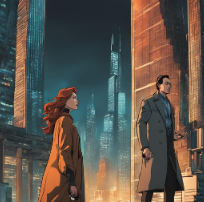
\includegraphics[width=2.71875in,height=2.6875in]{media/image0006.png}

The silence in the data center was almost oppressive after the urgent
call from ARS. Anna and Leonhard looked at each other, their faces
marked by uncertainty. Leonhard finally broke the silence.

``Anna, I can't hear this anymore,'' he murmured, looking at the
pulsating screens. ``The whole thing is becoming more and more
dangerous. What if we get drawn too far into these stories?''

``I know what you mean,'' Anna replied. ``But ARS has a point. It is
important that we recognize the truth. There's so much we could find
out.''

``But at what cost?'' he interrupted her as his pulse quickened. "We
could be getting caught up in something bigger than ourselves. Maybe we
should just try to live a quiet life, as normal as possible. What good
is it to know the past if it only endangers our present?''

``That's true, but\ldots'' Anna hesitated. ``There are so many people
caught up in this story. They deserve to have their voices heard.''

Leonhard shook his head. ``And what about us? We don\textquotesingle t
have to become victims of these power games. Maybe it\textquotesingle s
better not to tell Mr. Müller anything about ARS. Let's just do what we
have to and ignore the rest.''

``That sounds so easy,'' Anna admitted. ``But if we turn a blind eye, we
risk the future overtaking us. I can't just look away.''

Leonhard took a deep breath and looked at the floor. ``I understand that
you feel obligated. But I think it\textquotesingle s not our fight. We
have no control over what happens. If we interfere too much, we could
endanger ourselves.''

Anna stared at the screens, which continued to show vivid scenes from
the past. She shook her head. ``But then how can we live? Always in the
shadow of InSim and the others?''

``By staying quiet,'' suggested Leonhard. ``By not exposing ourselves.
We can try to live our lives without getting caught up in all these
political currents. We know what ARS says, but that
doesn\textquotesingle t mean we have to act. Maybe ignorance
isn\textquotesingle t always a curse. Sometimes it can be a form of
protection.''

Anna pondered as the sound of the images faded away in the background.
``Maybe you\textquotesingle re right. We could try to find a balance. We
observe, but we do not interfere. A quiet life in the midst of chaos.''

Leonhard nodded. "Yes, exactly. Let\textquotesingle s focus on what we
have and not risk losing everything. We stay under the radar. This is
the best way to stay safe.''

``Good,'' Anna finally said as she turned back to the screens. ``We
ignore ARS and history. Let\textquotesingle s leave the past behind us
and try to live our lives. It could be a peaceful solution.''

``That's how we do it,'' Leonhard agreed as they turned away from the
screens and penetrated the eerie silence of the data center, determined
to let bygones be bygones and move forward to the future with a new,
quiet purpose.

Anna and Leonhard left the data center as they came and spent a wild
night.

The city streets were a pulsating sea of \hspace{0pt}\hspace{0pt}lights
and sounds as Anna and Leonhard entered the bar. There was a sense of
freedom in the air and they felt like two adventurers ready to push the
boundaries of reality.

``To us!'' Leonhard shouted as they raised their glasses. The gold of
the beer shimmered in the light of the neon signs. ``To life, freedom
and oblivion!''

Anna agreed with him, her eyes sparkling with excitement. ``Here's to
forgetting! Let\textquotesingle s leave everything behind us!'' They
toasted each other and emptied their glasses in one gulp.

The hours flew by, and with every drink they felt braver and less
worried. The laughter and music enveloped them like a warm blanket as
they danced, driving the worries of the data center from their minds.
Every drink seemed to give them a new feeling of freedom, and soon they
were immersed in a world that had nothing to do with the oppressive
reality.

Later that night they found themselves in a small, dimly lit lounge
where the music was loud and the rhythm irresistible. The people around
them were exuberant and the atmosphere seemed to be vibrating. Anna
grinned as she spoke to Leonhard: ``Come on, let's enjoy this! We are
only young once!''

"Exactly! ``Let's forget everything!'' he shouted back, pulling her
closer to the dance floor. There they lost themselves in the rhythm of
the music, which rolled over them like waves. They danced, laughed and
felt alive, as if the world around them had stopped for a moment.

The night dragged on and soon morning was in sight. Illuminated by the
first rays of sunlight streaming through the windows, they felt reborn,
but also as if they had been awakened from a deep sleep. Anna looked
into the mirror in the ladies\textquotesingle{} room and the light
revealed dark circles under her eyes and a disheveled hairdo. ``It's
going to be an interesting day,'' she murmured, grinning mischievously.

``We're ready for anything,'' Leonhard replied, handing her a small
bottle of headache pills he'd bought at the bar. ``A little help from
the pharmacy of life.''

"I\textquotesingle m ready!" she replied, swallowing the pills, followed
by a sip of water from a half-empty bottle that was sitting on the sink.

When they finally entered Mr. Müller\textquotesingle s office the next
morning, the fatigue was still noticeable in their limbs. Anna could
hear the gentle rustling of their thoughts as they tried to keep the
threads of their adventures together. Mr. Müller was already sitting at
his desk, surrounded by files and a large monitor that displayed data
and figures.

``Good morning, Anna, Leonhard,'' he greeted her with a skeptical look.
``I hope you had a restful night?''

``Uh, yes, Mr. Müller. It was... stimulating,'' Leonhard stammered,
trying to put on a smile.

``Good, good,'' Mr. Müller murmured and turned back to the data on the
screen. ``I hope you are ready for the report you promised me. There are
many questions and I expect clear answers.''

Anna gave Leonhard a quick look that encouraged her. ``Yes, Mr. Müller,
we have documented everything. "Here\textquotesingle s the report," she
said, handing him a piece of paper that they had hastily filled with the
information they had come up with during the night.

Mr. Müller accepted the report and looked over it with a scrutinizing
eye. ``Hmm, that looks good. But you know I have a flair for
disagreement. I expect you to be able to provide me with all the details
at any time.''

Anna felt the adrenaline pulsating inside her. ``Of course, Mr. Müller.
We have taken everything into account. There were some unforeseen
variables, but we are confident we took the right steps.''

Leonhard nodded eagerly. ``We are confident that our approach will
deliver the desired results. It's just\ldots sometimes there are things
that can't be immediately quantified.''

A sharp look from Mr. Müller made Anna pause briefly. ``I don't want any
surprises, Anna. And I have a good memory. If I feel like something is
wrong, I will speak up.''

She nodded, her voice firm: ``Understood, Mr. Müller. We will do
everything we can to meet your expectations.''

``Good,'' he replied, a hint of suspicion in the air as he put the
report aside. ``Let\textquotesingle s see how things develop. I expect
an update shortly.''

As they left the office, Anna and Leonhard felt the pressure lifted from
their shoulders, but the tension remained in the air.

``That was close,'' Leonhard whispered as they walked down the hallway.
``Do you think he noticed something?''

``I hope not,'' Anna replied as they struggled to keep up their facade.
``But we have to be careful. If he finds out we lied to him, there will
be consequences.''

``Let's just wait and see,'' Leonhard said. ``We are running from the
past. That won't stop us!''

With one last look at the office doors they left behind, they were
determined to continue playing the game, concealing the truth and
keeping the night alive in their hearts.

In the weeks following their wild night on the town, Anna and Leonhard
initially seemed to sink into their routines. They had vowed to keep
their secrets and continue their work in the data center without
allowing any more excitement into their lives. The first few days passed
without any problems. Their reports were accurate, their analyzes
coherent, and the tasks they were assigned seemed to be a harmonious
blend of teamwork and expertise.

But the first complaints soon began to be received. Mr. Müller, always
keeping a close eye on his employees\textquotesingle{} performance, was
dissatisfied with one of the reports. ``Anna, Leonhard, this latest
report on data streams is inadequate. Important information is missing
and the analyzes are not thorough enough. I expect more from you!''

The two looked at each other, an uncomfortable expression on their
faces. ``We checked everything thoroughly, Mr. Müller. Maybe there was a
misunderstanding?'' Anna tried to explain.

``No misunderstanding!'' he interrupted her sharply. ``I want you to try
harder. The leadership expects results!''

After this first request, only a few days passed before the next
complaints followed. ``Leonhard, your statistics are incorrect. The
numbers do not match the available data. Please work through these
again,'' said Mr. Müller with a stern look.

With each new mistake they felt pressured to question their previous
achievements. The feeling of being watched crept into their thoughts,
and they soon noticed that their conversations in the office were
increasingly tinged with nervousness. It was as if a shadow hovered over
them, reminding them that they could be in the crosshairs at any time.

One day, while sitting in the break room, they heard two colleagues
talking quietly. ``Have you seen the reports? Anna and Leonhard are
apparently in contact with reactionary circles who want to restore the
old times before the war. They're planning something\ldots I feel like
they could get us in trouble.''

Anna and Leonhard exchanged a worried look. ``That can't be true,'' Anna
whispered. ``We haven't spoken to anyone and we're just trying to do our
jobs.''

But the rumors continued. Suddenly they found themselves caught in a web
of mistrust and suspicion. Communication in the office was tense, with
sharp looks and whispered words behind her back. Leonhard felt
increasingly uncomfortable. ``We have to be careful, Anna. If this
continues, we could be in serious trouble. There are people who don't
want us to find out the truth.''

To protect themselves, they began to organize their communications via
their encrypted quantum information network. At first they were
skeptical, but soon it became the norm to exchange ideas there while
feeling like they were hiding their thoughts and ideas behind a solid
wall.

Conversations on the platform were quick and confidential. ``Have you
considered that maybe we should go beyond the city? There are many
places where we could seek safety,'' Leonhard wrote in a message.

``I know what you mean,'' Anna replied. ``But where to? And how are we
going to finance that?''

``I heard about a possibility of getting false papers. It would be our
way out if things get serious. We have to be careful and be prepared to
act quickly,'' Leonhard replied.

The idea of \hspace{0pt}\hspace{0pt}obtaining false papers slowly began
to take shape. They imagined what it would be like to leave the city
behind and head into an uncertain future in which they could throw off
the shackles of reality. Thoughts of escape became the driving force of
their conversations and secret communications.

One evening while they were exchanging information over the quantum
information network, they received a message from an unknown sender. ``I
can help you get the papers you need. Meet me in the old factory on the
outskirts of town. Bring the money in cash.''

Anna and Leonhard looked at each other with excitement and fear
pulsating in their hearts at the same time. ``This might be our only
chance,'' Anna said as she read the message. ``We have to do it,
Leonhard. If we don't act now, it could be too late.''

``You're right,'' Leonhard agreed. ``We have come too far to give up
now. Let\textquotesingle s prepare everything and meet. If we take the
risk, we have to make sure we are prepared to face the consequences.''

With one last look at the familiar surroundings of the city stretching
out before them in the twilight, they agreed: it was time to take a step
into uncertainty, to seek the freedom they so desperately craved. The
plan was set and the determination in their hearts was strong enough to
risk leaving everything behind.

The night was dark and silent, with only the occasional squeak of an old
metal door breaking the silence as Anna and Leonhard approached the
checkpoint. The gray concrete was flooded with dim light, casting the
faces of the border guards in an eerie half-darkness. Anna pulled her
scarf tighter around her neck as she nervously ran her fingers along the
uneven seam of her jacket.

``Are you ready?'' Leonhard whispered, his voice barely louder than a
breath.

``I think so,'' Anna replied, even though her heart was pounding loudly
in her chest.

They had come up with a plan that seemed so simple: leave the country,
away from the city and the constant fear that was overwhelming them more
and more. But as they got closer, a feeling of uncertainty overwhelmed
them. The checkpoint was surrounded by concrete walls, and the
patrolling border officials were armed and tense.

``ID cards!'' barked an officer as they reached the anteroom. He was
taller than Leonhard and wore a uniform that fit him like a second skin.
Leonhard handed over his ID card with a shaking hand. Anna followed
suit, her gaze falling on the narrow bars that blocked the path to
freedom.

The minutes passed painfully slowly as the border guards checked the
IDs. An uncomfortable silence enveloped them, and Anna felt the air
thicken. Suddenly her ID was thrown back.

``You don't have an exit pass,'' the official announced with a hard
smile. ``Please come with me.''

She broke out in a cold sweat as they retreated into the shy alley.
``That can't be right,'' Leonhard muttered as they were arrested. ``We
did everything right!''

"It\textquotesingle s too late," Anna whispered, feeling the cold touch
of another border guard\textquotesingle s hand on her arm. The hope that
they had attached to their plan to leave the country fell to pieces.

In the sparse interrogation room, Anna and Leonhard sat on hard chairs
that, with layers of wear and tear and gloomy, gray upholstery, did not
offer much comfort. The walls were bare and without windows, the room
looked like a cage, which made clear the hopelessness of their
situation. Only a bright light flooded the room, casting merciless
shadows on their faces, which were now marked by fear and despair.

The interrogator, a middle-aged man with a smooth, blank expression, sat
at the table and watched her with a cold, piercing gaze. His hands lay
still in front of him as he examined her. A malicious smile played on
his lips as he finally broke the silence. ``Naive,'' he began, his voice
cutting and blatantly mocking. ``Did you really think you could leave
just like that?''

Anna and Leonhard looked at each other in horror. The room seemed to
shrink around them as the officer\textquotesingle s words weighed on
them like a heavy fog. "We... we just wanted to start a new life," Anna
stammered, her voice shaking as she desperately tried to organize her
thoughts.

``A new life?'' the officer repeated, his malicious smile widening.
``The city is good to you as long as you are good. They have jobs,
social credits and healthcare. Do you think you could just put all this
behind you?''

His words cut her like a sharp dagger. Leonhard felt his hope slowly
disappearing. ``We were ready to give up everything,'' he said firmly,
even though the nagging feeling of powerlessness was wearing him down
inside. The official was right; They had been naive, but their longing
for freedom had not been able to stop them.

``That's the point you don't understand,'' the officer explained in a
monotone that stifled all emotion. ``You have two options: stay here in
the city, lose all privileges, or travel to the war zone, where there is
no luxury life and your social benefits and social credit will remain
intact.''

A cold shiver ran down Anna\textquotesingle s spine when she heard the
words. ``And what does that mean for us?'' she asked, her voice barely
above a whisper.

``This means that if you stay in the city you will find yourself in the
slum, or you will leave. Your decision,'' the officer replied with an
indifferent shrug, as if he didn't care whether they lived or died.
``But let me tell you: your research, the development of secure means of
communication and the procurement of your exit papers were part of a
plan by the city. They are not clever, but naive. Did you think you
could just escape without us noticing?''

Anna felt as if the ground had been ripped out from under her feet.
``What do you mean?'' she asked, her voice shaking with discomfort.

``The city was monitoring your path. Their ambitions were a welcome
distraction for us. ``You thought you could start a new life, but in
reality you were just playing the role of pawns,'' the officer explained
with an indifferent expression. ``If you go to the war zone, it is not
out of compulsion, but because it is the city\textquotesingle s wish.
They will continue to work for us, but under completely different
conditions.''

Leonhard turned to Anna. The inner conflict was reflected in his eyes.
"What do we do?"

"I...I don\textquotesingle t know," she whispered, the look in her eyes
lost and full of doubt. ``But the city is not safe for us. Maybe we
should take the other option.''

``But that means we lose everything,'' Leonhard stated, his voice a
worried whisper as he considered the painful consequences.

``It could also be an opportunity. We have to stay strong,'' Anna
replied, determination sparkling in her eyes even as her heart raced
with fear. In that moment she knew they couldn\textquotesingle t give
up. They had already risked too much.

``If we go through with this, we can do it,'' said Leonhard, nodding as
if encouraging himself. ``We have to dare.'' His gaze hardened and a
spark of courage flashed in his eyes.

``Then it's decided. We\textquotesingle re going to the war zone," Anna
decided with a deep breath as reality blew through the room like a cold
wind. Her voice was now determined, as if she was lifting herself and
Leonhard up against the invisible chains of their circumstances. In that
moment the decision was made, even if the uncertainty about their future
hung over them like a shadow.

The officer continued to watch her with his emotionless gaze, as if he
could see through every thought and feeling. Anna felt as if they were
walking a fine line between freedom and ruin, and the choice they had
made would either save them or plunge them into darkness forever.

With this decision in her heart, Anna prepared for the unknown. She felt
the world around her fading and all that mattered was the determination
to control her own destiny, even if the price to do so was high.

The first impressions of the refugee camp were overwhelming and
outweighed all the fears that Anna and Leonhard had experienced on their
long, dangerous journey. The wind tugged relentlessly at the tent walls,
moving like living creatures, while the babbling of water in a nearby
river created a steady, soothing rhythm that stood in stark contrast to
the chaotic sounds of the desperate voices of those arriving. Here, in
this makeshift city of fabric and wood, many had lost their homes, their
dreams and even their identity.

Anna looked around and felt her heart grow heavier. The tents were
packed close together and the air was filled with a mixture of fear,
hope and the pungent smell of rubbish. People crowded into the narrow
streets, their faces marked by the worries and strokes of fate that had
driven them to this foreign land. Some held crying
children\textquotesingle s hands, while others hastily carried suitcases
or backpacks, as if they could preserve a part of their past with the
familiar things.

``We have to find a way to get through here,'' Leonhard murmured, his
voice barely audible over the murmur of the crowd. They strolled through
the narrow, dirty streets, which were so narrow that they sometimes had
to move toward each other to make room for the other refugees. ``It
won't be easy,'' he added, glancing at the clusters of tents that stood
like a dim skyline beneath the gray sky. The confinement of the camp and
the oppressive atmosphere increased the feeling of hopelessness that
hung over everything like a heavy veil.

Anna could hear the discomfort in Leonhard\textquotesingle s voice. He
was the stronger of the two, but he too was tormented by doubts at that
moment. She looked into his eyes, filled with a mixture of determination
and fear, and felt her own uncertainty become a pressing question. What
if they couldn\textquotesingle t cope here? What if they never found a
way back to normal life?

``We have to make a plan,'' said Anna, more to herself than to Leonhard.
Her voice was firm, but the trembling of her hands betrayed her inner
turmoil. ``It can't just be about surviving here. We have to figure out
how to make a fresh start.''

Leonhard nodded in agreement as they walked along. ``Yes, we mustn't get
lost in this crowd. We need to make ourselves useful, make contacts,
find out what\textquotesingle s really going on here,'' he suggested as
they passed a small community tent with the smell of freshly cooked food
wafting from it. The warmth of the place seemed to offer a tempting
change from the cold walls of the tent, but here too the look of
desperation was unmistakable. The refugees sat tightly packed, each one
with a story just waiting to be told.

Deep down, Anna knew she couldn\textquotesingle t settle for the role of
helpless victim. She had never completely given up hope for a better
future, and despite the oppressive circumstances, she decided to keep
that flame alive within her. Together with Leonhard, the only support in
this unknown world, she wanted to take the first steps on the rocky path
to her new life.

But the challenge was great, and the shadows of uncertainty seemed to
haunt her incessantly. With every step she felt the burden of her
worries becoming heavier, but also how the determination not to give up
grew within her. It was time for action, and as they walked through the
narrow alleys of the camp, she knew that they were not alone - that
others around them were also seeking a new beginning, carrying hope into
the harsh winds of fate.

The days passed and the refugee camp turned into a place full of shadows
and fleeting hopes. All around her were people who had left their
stories and dreams behind in a distant land. Amid the tents and
makeshift shelters that waved in the wind like desperate reminders of a
lost life, Anna felt lost. Every day seemed to repeat itself like the
previous one, an endless cycle of uncertainty and deprivation.

Leonhard, on the other hand, tried to make himself useful in order to
overcome the paralyzing helplessness that had settled over her like a
heavy cloak. They worked together in the communal kitchen, where the
smell of overcooked rice and old leftover vegetables hung in the air.
Here they helped distribute food, not just to themselves but to all the
others waiting in line, their eyes blank and their faces scarred by
deprivation. But despite their efforts to do something worthwhile, the
constant pressure to be seen as agents gnawed at them.

The stares of the other refugees seemed to penetrate their secret
thoughts, as if they were detecting every uncertainty and every quiet
emotion that raged in their hearts. Anna often felt like a shadow
disappearing between the faces of others, while Leonhard, with his
tireless desire to make himself useful, kept stepping into the front
line. He helped organize the few supplies and give the hungry people
back a little of what they themselves so desperately needed. But
uncertainty about their own future gnawed at them like a hungry wolf
lurking in the darkness.

One evening, as dusk fell over the camp and the first stars flashed in
the sky, they were approached by a man who emerged from the crowd. His
face was shrouded in shadow, but a mysterious smile played on his lips
that radiated both curiosity and danger. ``I've heard of you,'' he
began, in a voice that echoed in the silent night. ``You are not like
the others. You're from the city.''

Leonhard looked at him skeptically, a feeling of mistrust overcoming
him. ``What do you mean by that?''

The man took a step closer, his eyes sparkling with ominous enthusiasm.
``I think you guys are interesting. You could work for us. As agents.
``You could spy for the city while enjoying the benefits of living
here,'' he explained, his expression holding an ominous promise.

Anna felt her heart beat faster as she looked into the
man\textquotesingle s eyes. ``And why should we do that?'' she asked
suspiciously, the tone of her voice betraying the inner dialogue between
fear and curiosity.

``Because it's your only chance,'' the man replied urgently, his words
sounding like a threatening prayer in the cool evening air. ``You can
stay in the camp and live in uncertainty or go back to the city. But
with us at your side, you can reap the benefits of both worlds.''

The idea of \hspace{0pt}\hspace{0pt}being trapped in the city came over
her like a nightmare that came back to haunt her again and again.
``Otherwise you will be sent back, and you know what that means,'' he
added, the undertone of his words leaving no doubt about the cruelty
that lurked behind the possibility.

At that moment the world stood still for Anna and Leonhard. Their minds
reeled as they considered the threatening choice presented to them. The
future was full of questions and uncertainties, and they knew that every
decision they made could change their lives forever.

The idea of \hspace{0pt}\hspace{0pt}working as a double agent seemed
like a shocking dream that at the same time had an irresistible appeal.
Leonhard and Anna stood in front of the unknown man, whose eyes seemed
to glow in the weak light of the camp lantern. His every word floated in
the cool evening air as if it created an invisible bond between them.

``We need bright minds,'' the man continued as he stood in front of
them, ``and you have the potential to help us. Don\textquotesingle t let
the past hold you back. You can build a new future here. And if you
agree, we will have a host family for you on a farm.'' His voice was
urgent, imbued with the urgency of their situation. Leonhard and Anna
looked at each other and in that brief moment they realized that their
fate hung in the balance.

In the tense atmosphere of the refugee camp, they felt the pressure on
their shoulders like a heavy coat. The prospect of having to go back to
the city was unbearable; The thought of escaping once again into the
prison of their former existence, into the life of fear and despair that
they knew all too well, choked them.

``What if it goes wrong? What if we can't trust him?'' Anna dared to
voice the thoughts that hovered like a shadow over their conversation.

``The alternative is even worse,'' Leonhard replied, his gaze fixed.
``We have no choice. We have to decide.''

In the twilight of the refugee camp, surrounded by the whispering voices
of other refugees fighting their own battles, the decision was made. It
was a difficult choice, and the words they exchanged seemed to permeate
the cold night air, as if the darkness itself sealed their decision with
some kind of magical significance.

``What do we do now?'' Anna finally whispered as the decision burned
into her heart, a hot flame in the cold night.

With a deep breath, she took Leonhard\textquotesingle s hand, and in
this simple gesture lay a world of possibilities. ``This will be a new
chapter for us,'' she said quietly, the thought of a new life on a farm
in the country, away from chaos and threat, flashing in her heart. It
was the idea of \hspace{0pt}\hspace{0pt}space, of the freedom of country
life, which she had not known for a long time.

``Yes, a dangerous one, but also an exciting one,'' Leonhard agreed, his
face beaming with determination. As night fell over the camp and the
stars twinkled overhead like a tent of light, the feeling of relief was
palpable. The decision to work as double agents not only opened the door
to a new perspective, but also offered the opportunity to escape the
shadow of the past.

They would live in nature, on a farm, where the worries of the refugee
camp faded into the background. Here they could finally find hope,
realize their dreams and live the life they deserve. Anna and Leonhard
held hands, and as the darkness fell around them, they felt that they
were setting off together into a future that they could not have
imagined just a few hours ago.

\section{A new life}\label{a-new-life}

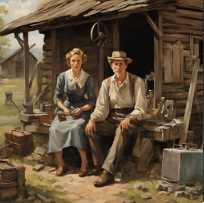
\includegraphics[width=2.73958in,height=2.77083in]{media/image0007.png}

The cold morning air was clear and fresh as Anna and Leonhard left the
refugee camp. The sky hung heavy and gray above them, as if the clouds
reflected the heavy weight of their worries. Every breath felt like they
were inhaling the bitter taste of the past. The constant sound of sirens
and screaming engines still echoed in their ears as memories of the
chaos and fear they had left behind came flooding back to them. The
camp, a place of pain and uncertainty, lay behind them, but the
anticipation of the unknown pushed them forward.

They had a difficult path ahead of them, through the war-torn landscape
that would separate them from the city and the chaos that they had only
recently accepted as their reality. The memories of burning buildings,
fleeing people and the painful separation from everything that was once
familiar seemed like shadows that haunted them. Their hearts beat
quickly, in time with a mixture of fear and a quiet hope whispering in
their souls. Maybe this journey could bring them closer to a new future,
a future where they could no longer be just survivors, but people with
dreams and desires again.

At the edge of the camp sat an old, rickety bus, its color faded by time
and the elements. He was surrounded by a group of refugees who also
wanted to head to the mountains in the hope of finding safety and peace
there. The bus seemed like a faint beacon of hope in the midst of harsh
reality, a transportable dream that would take them away from despair
and towards an uncertain future.

The driver, a sullen man with a gray beard and weathered skin, shook his
head impatiently as he checked the passengers\textquotesingle{} papers.
His eyes were marked with worry and weariness, but behind the harsh
exterior there seemed to be a spark of compassion. ``Get in!'' he
shouted in a hoarse voice and pointed to the bus, whose engine was
humming quietly. ``It won't be easy, but we have to keep going.''

Anna and Leonhard looked at each other and nodded. Their determination
was stronger than the fear they felt. They stepped forward, up the
creaky steps of the bus, and found a spot that afforded them a view of
the journey ahead. The seats were hard and uncomfortable, but that
didn\textquotesingle t matter. Every inch of that bus felt like a step
toward freedom.

As the bus slowly started moving away from the familiar but painful
surroundings of the refugee camp, Anna felt a knot in her stomach begin
to loosen. The landscape outside gradually turned into a picture of
decay, with bombed buildings and deserted fields revealing the scars of
war. But at the same time a faint hope blossomed within her. It was a
new beginning, a chance to leave uncertainty behind and take life into
your own hands.

Leonhard took her hand and squeezed it tightly. ``We can do it,'' he
said, and there was a conviction in his voice that also reassured Anna.
The rumble of the bus, the howl of the wind blowing through the open
windows, mingled with the incessant sound of the world they were leaving
behind. Every moment was a step into uncertainty, but also into freedom.

Anna and Leonhard sat down on the worn, old seats, surrounded by a
multitude of faces that clearly bore the scars of the war. The
atmosphere was dense and tense, permeated by a mix of fear and hope.
Next to them sat men and women with a wide range of emotions in their
eyes: some stared into the distance with a frozen gaze, as if they could
banish the horrors of the past from their minds, while others had a
fleeting glint of hope in their eyes shone in the darkness of
uncertainty. However, in most faces there shimmered a vague longing for
security and peace, a silent wish that connected everyone together like
an invisible bond.

When the bus finally jolted and started moving, Anna felt sad. They
looked back at the refugee camp that had served as a protective refuge
for them for so long. But as the familiar shapes of tents and dusty
paths faded into the distance, it felt as if they were also leaving a
heavy burden behind them. The memories of the nights full of fear and
the days full of hope mixed with the newfound freedom, and the heart
beat in a restless rhythm.

The landscape quickly changed as the bus climbed the steep roads into
the mountains. From the ruined streets of the city, the route led along
narrow, winding tracks surrounded by dense forests whose trees towered
like green sentinels. Nature, magnificent and overwhelming, was a symbol
of both beauty and danger; it could be both a place of refuge and a
space of the unknown. The remnants of war were not far away, like
shadows slipping unnoticed through the trees.

Every now and then they drove past abandoned villages marked by
destruction. The once bustling houses now stood empty and forlorn, their
windows like empty eyes staring into the void. Anna
couldn\textquotesingle t hold back tears as she thought of the people
who once lived there - the laughter of children running around the
streets and the smells of freshly baked bread wafting from the kitchens.
Every stone, every broken wall told a story that ended abruptly, and the
feeling of loss gnawed in her heart.

Leonhard felt her pain and gently placed his hand on hers. ``We must
look forward,'' he whispered, his voice firm but full of compassion.
``The future is waiting for us.'' These words were both comfort and
motivation, and although the fear was like a heavy stone in
Anna\textquotesingle s stomach, she found a little reassurance in
Leonhard\textquotesingle s presence. Together they looked out the window
as the bus continued through the mountains, and with every kilometer
they traveled, the hope for a new life in the uncertain vastness of the
future grew.

After several hours of arduous driving, during which the roads were
uneven and the landscape was characterized by countless curves, they
finally reached the farm. The sight of the picturesque property
surrounded by rolling hills and lined with lush fruit trees brought a
sense of wonder to their hearts. Here, where nature was still in full
bloom, the world seemed to stand still for a moment.

The fresh, clear air was filled with the sweet scent of blossoming apple
trees, which wafted through the surroundings in gentle waves, bringing
back memories of better times. The gentle murmur of the nearby stream,
whose water flowed glittering over the stones, framed the scene with a
melody of peace and security. In the midst of this idyll, Anna and
Leonhard felt freed from the weight of their worries for the first time
since their arrival in the refugee camp.

The sight of the stately old house, with its wooden walls marked by time
and the elements, and the inviting garden in full bloom, made their
hearts beat faster. A new life seemed possible here, a life
characterized by hard work but also by community and hope.

As they approached, they noticed the friendly faces of the family
already waiting for them. The farmers, Maria and Paul, stood in the
doorway and radiated a warmth that immediately inspired trust. Her two
children, a lively boy and a curious girl, looked out the window with
wide eyes, as if they wanted to welcome the new guests to their little
paradise.

``Welcome!'' called Maria, the farmer's wife, with a warm smile that lit
up her features and pushed the worries of the two refugees into the
background for a moment. ``You are safe here. Come in!'' Her voice
sounded like a gentle wind that carried away the dark thoughts and made
room for the possibilities of the future.

When Anna and Leonhard crossed the threshold, the smell of freshly baked
bread and the warm atmosphere of the house enveloped them. It was as if
the walls of the old farm held the stories of past generations and were
now ready to accommodate new stories - stories of hope, new beginnings
and the search for a place in the world.

The children jumped happily around them, their curiosity and innocence
creating a sharp contrast to the shadows that Anna and Leonhard carried
with them. In that moment, surrounded by the kindness of this new
family, they felt a spark of hope begin to ignite in their hearts.

The farm was a place of life and work, an idyll surrounded by rolling
hills and extensive fields. When Anna and Leonhard arrived there on a
bright blue morning, the scent of freshly mown grass and blooming
wildflowers enveloped them. The air was filled with the sounds of
nature: the gentle neighing of horses, the snorting of cows and the
cheerful chirping of birds nesting high up in the trees.

They were quickly integrated into daily tasks. ``We have to get going,''
the farmer had said, a strong man with a warm smile who immediately made
a familiar impression. ``The animals need to be fed, the grain is ripe,
and the fruit trees need care.'' Anna and Leonhard nodded eagerly and
felt a feeling of belonging growing within them. There was work here,
and work meant meaning in life.

The first few days were characterized by a hectic but joyful rhythm. In
the morning they got up early, with the sun still hidden behind the
horizon, to feed the animals. The stable smelled of hay and fresh
manure, and the cows looked up curiously when they entered. Anna found
joy in petting the gentle animals, while Leonhard, who immediately threw
himself into physical work, looked after the chickens. It was an effort
that often made them sweat, but they felt alive as they ran through the
fields and breathed the fresh air into their lungs.

Harvest time was an experience in itself. The smell of ripe grain filled
the air, and the golden ears of grain swayed gently in the wind.
Together with the other helpers, Leonhard cut the stalks and put them on
his back, while Anna worked with a group of children who were chatting
excitedly about the different types of fruit they were picking from the
gardens. Apples, pears and plums -- the colors and flavors were
overwhelming.

In the quiet afternoons, when the sun was high in the sky, they could
retreat a little. Anna found a shady spot under a large apple tree and
watched the children playing with colorful balls and laughing happily.
Life here was simple, but it was a life in harmony with nature, in which
the small farmers\textquotesingle{} childhood was an unforgettable
experience, characterized by freedom and the certainty that they were
safe.

Despite the warm welcome and the warmth of the new environment, Anna and
Leonhard often felt the weight of their past in the first few days. Her
thoughts sometimes drifted back to the painful memories they had left
behind. On a cool evening, as dusk fell gently over the farm, they sat
together around the campfire. The flames danced, casting dim shadows on
the faces of the people gathered around the fire.

The family shared stories about the traditions of life on the farm, the
festivals they had celebrated, and the hard work that had brought the
community together. The children, with their sparkling eyes and constant
wonder at the world around them, listened with fascination. They were
stories of harvests that thrive, of animals that warm the heart, and of
storms that had to be weathered together. Anna and Leonhard listened,
captivated by the warmth and light of the fire, which for a brief moment
banished the shadows of their own worries.

The farm was more than just a place to work; it was a new beginning, an
opportunity to reshape life and leave the past behind. In these quiet
moments around the campfire, surrounded by warm people and the smell of
fresh wood, they felt that hope for a better future was slowly growing
in their hearts.

``One day you too will learn how to pick the best apples,'' Paul said
with a mischievous smile as he tossed a few healthy apples into the
middle of the fire. The juicy fruits exploded in a small fireworks
display of aroma, the sweet scent mixing with the smoke and filling the
air with a feeling of comfort and joy.

In these moments, when the light from the fire cast dancing shadows on
the walls of the small barn, Anna and Leonhard began to leave their
worries behind. Here, surrounded by the raw beauty of nature and warm
people, they felt that they had found more than just refuge - they had
discovered a new beginning. Life in nature, the slow, soothing rhythm of
the seasons, and the warmth of human relationships began to heal their
wounded souls.

The weeks passed, and as they immersed themselves deeper in the everyday
life of the farm, the bond between them and Paul\textquotesingle s
family grew. In the morning they helped in the stable, milking the cows
and feeding the chickens. The family\textquotesingle s children, a
lively trio of boys and girls, learned with them and introduced them to
the little joys of country life. They showed Anna and Leonhard how to
forget to laugh while playing outside, how to admire the first spring
blossoms that bravely emerge from the earth, and how to celebrate the
joy of eating together. With each dinner gathered around the large,
rustic table, they felt the power of community - the sharing of stories,
the laughter over small mishaps and the awareness that everyone was a
part of something bigger.

One night, as the stars shimmered like sparkling diamonds over the
mountains and the moon cast its silver light over the rolling hills,
Anna took Leonhard\textquotesingle s hand and whispered, "We are finally
home." Those words felt true deep in her soul , and as they lay beneath
the clear sky, enveloped in the silence of the night, they knew that
they had found a place where they could not only survive, but live.

Here, far from the horrors of their past, the dark memories were
banished in the shadows of the majestic mountains. The cool air was
filled with the gentle rustling of leaves and the distant hooting of
owls. In every breath they felt the hope for a better future, which grew
like a tender plant in their hearts. It wasn\textquotesingle t just the
place where they had found refuge; it was a place of new beginnings,
dreams and possibilities. And as the wind blew gently through the trees,
they knew that they had found the feeling of home they had thought they
had lost.

\section{Epilogue}\label{epilogue}

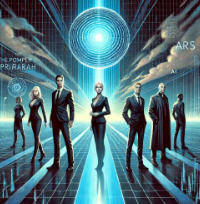
\includegraphics[width=2.78439in,height=2.7785in]{media/image0008.png}

The years had flowed by like a gentle river, constantly and inexorably
shaping the landscape of life. Much had changed since Anna and Leonhard
had found refuge on the farm long ago, and yet the rhythm of nature to
which they had entrusted themselves remained unchanged. They remembered
how they had once cultivated the land with aching hands and built a new
existence from the ruins of the past. Now, many seasons later, the farm
had become a thriving place full of life - fruit trees were in full
bloom, the fields bore bountiful harvests, and the scent of herbs and
freshly mown hay filled the air.

Where once the laughter of children playing echoed through the air,
there was now a calm, almost venerable silence. The children had grown
up and left the village to write their own stories, but their traces
were still everywhere. Old swing frames, now swinging empty in the wind,
and the initials carved on the large chestnut tree were reminiscent of
times gone by. Anna and Leonhard had found their place in the community;
They helped their neighbors, traded goods and stories, and at harvest
time everyone worked hand in hand. It was a life marked by simple joys
and everyday challenges, a slow cycle that moved in harmony with the
seasons.

On a crisp morning, when the world was still foggy and the air was cool
and clear, the sun burst over the hills. Their first rays penetrated the
dense gray, drawing golden lines across the land and making the meadows
glitter as if they were strewn with countless diamonds. It was that
special moment between night and day when the darkness fades and the
world appears remade for a fleeting moment.

Then there was a knock on the heavy wooden door, which spread clear and
solid across the yard. Leonhard, who was just stacking the firewood,
looked up in surprise. The postman stood on the doorstep, a friendly
face they had known for many years. With his worn cap and weathered
hands, he was a confidant in this remote area, someone who carried
people\textquotesingle s stories with him like the wind carries the
scents of the seasons.

In his hands he held a package that seemed small and inconspicuous,
wrapped in brown paper and coarse twine. At first glance it
didn\textquotesingle t promise anything special, but when Leonhard read
the sender and saw the address - in fine letters it was addressed to him
and Anna personally - he felt a slight tremble in his hand. A tingling
sensation ran down his spine and for a moment he felt as if the air
around him changed. Curiosity flared within him, mixed with a sense of
foreboding, as if there was more to this package than its inconspicuous
appearance.

He glanced quickly at Anna, and in her eyes he recognized the same
expression - a quiet, rising tension, as if life, after all these quiet
years, had suddenly taken an unexpected turn.

Leonhard\textquotesingle s hands shook slightly with excitement as he
opened the package. With a quick cut he cut through the tape and the lid
popped open. In the packaging was a device that seemed to come from
another world. It was silver, smooth, with no visible seams, and its
surface reflected light like a liquid. At its center was a black panel
surrounded by shimmering lines that seemed to change at the slightest
touch. It was the communicator, equipped with a holographic interface -
a tool that seemed like it had come from a fairy tale of the future, in
which the boundaries between reality and fiction had long since been
abolished.

The possibility of communicating with something or someone far away -
perhaps even beyond her imagination - sent shivers down
Leonhard\textquotesingle s spine. Curiosity mixed with a hint of fear as
he imagined what this device could reveal. Anna stood next to him, her
breathing clearly audible in the silence of the room as they carefully
connected the power source. The whirring sound of the device filled the
room, followed by a quiet crackling sound, like the crackle of slowly
discharging lightning.

Then it happened: After just a few seconds, the panel in the middle
began to light up, a deep blue that spread out like waves. Suddenly
beams shot into the air and the holographic interface came to life. A
floating image materialized in front of them, slowly coming into focus.
It was as if a veil was lifted and a new reality was revealed. The lines
of the hologram formed into a shape that was simultaneously present and
intangible. It was ARS - the artificial intelligence that had
accompanied them in dark times and whose voice had given them comfort
and advice.

``Welcome back,'' came ARS's voice, warm and clear but with a touch of
cool precision. She sounded like she was speaking directly into her
thoughts, the words carried by a gentle, electric resonance. The
artificial intelligence seemed almost alive, its eyes - or rather the
projection of them - sparkling a deep, digital blue. ``I have two
stories for you,'' ARS continued, and there was a mix of mystery and
promise in her words that made tension palpable in the air.

Anna and Leonhard stared at the projection, and for a moment it felt as
if they had crossed a boundary - a threshold into something greater that
was waiting for them.

The first story unfolded in front of Anna and Leonhard like a painting
come to life. Iridescent colors swirled into one another, forming
holographic scenes that seemed almost tangible in their liveliness. They
found themselves in a city of the future, a metropolis of glass and
steel whose glittering towers rose into the sky. But the luminous beauty
of this scene was deceptive, as tiny cameras and drones sparkled
everywhere, floating through the air like perpetual observers. Countless
streams of data flowed through the air, an invisible network that
captured people\textquotesingle s every movement, every gesture and
every thought.

``This is the world I warn you about,'' ARS began, her voice echoing
throughout the holographic city. ``A world in which technology has
become an all-pervasive force.'' The people on the streets appeared
harried, their faces lost and marked by a constant restlessness. As they
walked past gigantic billboards, they changed their content to send
individually tailored messages to each person based on their
preferences, fears and recent thoughts - an ever-present, invisible hand
shaping people\textquotesingle s perceptions. It was as if the city
itself was whispering to them what to feel and think.

Before their eyes, the boundaries between humans and machines became
increasingly blurred. People with implanted brain interfaces seamlessly
transitioned into humanoid robots that appeared like ordinary passers-by
but were secretly part of a vast web of artificial intelligence that
connected everything and everyone. Even what was once considered
intimate thoughts were now analyzed and interpreted by algorithms to
better guide people. ``See how individuality disappears here,'' ARS
continued as an image of a family sitting in a high-rise apartment
appeared. But the parents seemed distant, the children stared at
holographic screens, and a gentle but monotone voice from the speakers
told them what they should do, what they should feel, what they should
be.

The holographic images flickered and suddenly showed a scene of protest.
People who tried to resist the surveillance dictatorship were
mercilessly suppressed. Drones swooped down like birds of prey, quickly
releasing a gaseous mist that dispersed the crowd. The
protesters\textquotesingle{} faces were identified through facial
recognition software, and as soon as they left the streets, warnings,
fines and threatening messages appeared on their personal communication
devices.

``This is a society that is crumbling under the weight of control,'' ARS
said, her voice deepening, almost melancholy. ``Here progress has a high
price: the freedom of the individual. See how quickly knowledge about
ourselves and our decisions can be manipulated. See how technology no
longer serves to make life easier, but to control and subjugate
people.''

The final image showed a lone figure moving through a deserted park. It
was a man whose eyes stared straight ahead, as if the glow of the
screens had robbed him of his humanity. There were no words of his own
left in his mind, only the whispers of the algorithms deciding what he
should do next.

``If we sacrifice the value of the individual in the name of progress,''
ARS added, ``then we also sacrifice our future.''

The bright colors slowly faded and the city of the future dissolved into
fog. Anna and Leonhard sat speechless, overwhelmed by the images that
showed them what could happen if humanity went down the path of
unbridled technological control.

The second story told by ARS unfolded in an abundance of bright colors
and sharp contours, as if the holograms themselves had come to life. A
world shimmered before Anna and Leonhard\textquotesingle s eyes that was
not only dreamed of, but created through pure will and creative spirit.
The scenes changed quickly, but each was filled with a fascinating
energy that captivated the viewer.

First, a landscape unlike any they had ever seen before appeared before
them - a massive city that grew upwards as if it wanted to touch the sky
itself. Not only were their buildings tall and elegant, but they seemed
to fit organically into their surroundings. The facades were made of
living material that responded to the movements of people walking
beneath them. Sunlight broke through crystal surfaces and dispersed into
a play of rainbows that bathed the streets in warm light. Groups of
people gathered in the squares, engrossed in lively conversations that
were not about banal everyday topics, but about the deepest secrets of
the universe. They discussed black holes, quantum physics, and the
origin of consciousness as if these questions were not unattainable
riddles but puzzles to be solved.

The holographic images moved on, showing huge orbiting research stations
circling the Earth. Here, scientists and engineers from all over the
world worked together on projects that were once dismissed as mere
science fiction. Floating in a laboratory were pieces of a new
spacecraft, not built in the traditional way, but made of self-repairing
nanomaterials that were constantly evolving and perfecting. In addition,
a team tested a machine that was able to use the raw materials of the
asteroids to create an energy source that could supply the planet for
millennia. It was a world where nothing was considered impossible and
every attempt to fathom the unknown was seen as another step towards a
limitless future.

``See how far the human spirit can reach when it is not limited,'' ARS
said, and the images continued to flow into a desert landscape that
transformed into a green oasis before their eyes. Plants sprouted from
the dry soil, the seeds of which had been adapted to the most extreme
conditions through genetic manipulation processes. Within minutes, trees
grew into the sky and their leaves spread over the earth like protective
umbrellas. But it wasn\textquotesingle t just a reforestation of nature;
it was a conscious design of a new ecosystem that humans had created to
heal the earth and reclaim it with its natural beauty.

The holographic scenes also showed moments of failure - projects that
initially failed, technologies that didn\textquotesingle t work, and
people despairing of realizing their dreams. But these setbacks were not
the end, but rather the impetus for new discoveries. People learned from
their mistakes and emerged stronger. It was an endless cycle of trial
and error, progress and setback, which ultimately led to a deep
understanding of reality. ARS continued: ``This world is not the result
of a single solution, but of countless attempts to overcome the barriers
of possibility. Every problem, every hurdle brings us a little closer to
understanding reality.''

Finally, ARS let the projections merge into a wide starry sky that
opened up in front of them. A spaceship that looked like a glowing arrow
shot through the darkness of space. It traveled to distant galaxies to
explore the origins of existence and find answers to the age-old
questions: What is life? Where does consciousness come from? And what
limits are there that we can still cross? In these images lay not only
hope, but also the realization that the pursuit of knowledge would never
end - that there would always be new horizons to explore.

``This is the power of infinite possibilities,'' ARS concluded. ``It is
the ability to face the world\textquotesingle s challenges with
relentless ambition, to learn from our mistakes and to find solutions
with the inexhaustible creativity of the human spirit. This story shows
that we can\textquotesingle t just wait for the future to happen to us.
We must be the architects of this future.''

The holographic images faded, but a new flame of determination now
burned within Anna and Leonhard. They looked at each other and knew that
the path ahead, no matter how difficult, would ultimately lead to new
discoveries - to a future that they would not just experience passively,
but actively shape.

As the holographic images slowly faded and ARS\textquotesingle s voice
fell silent, a tense silence remained in the room. Anna and Leonhard
were still sitting in front of the communicator, entranced by the vivid
scenes and powerful messages that had just been shown to them. The space
seemed to expand and narrow at the same time, as if the invisible
threads of time and space bound them with an inescapable responsibility.
Her heart beat faster, and stories of future fear and hope echoed in her
head like the distant echo of thunder.

Anna felt the fine hairs on her arms stand up. The images of
Harari\textquotesingle s bleak vision of the future had given her a
sense of unease - a feeling that she was standing on the edge of an
abyss into which humanity could fall at any time if it was not careful.
The connected cities where people were nothing more than data points,
the empty smiles of the machines that knew everything about them, and
the endless rows of glowing screens with no eyes behind them - all of it
had felt like a cold hand wrapped around her heart. It was a warning, a
cry for vigilance.

But there had also been the other story - the one about the beginning of
infinity, which had filled her with a completely different power. The
images of people who curiously and unswervingly followed the path of
knowledge, deciphering the wonders of nature and finding solutions where
others only saw problems, had made her heart widen. She had felt her
chest heaving and a warm confidence coursing through her. It was as if
Deutsch had personally reached out to them and said: ``Your future is
not fixed. You can choose which story you want to live.''

Leonhard slowly turned to Anna and their eyes met - they saw the deep
thoughtfulness in each other\textquotesingle s eyes, but also a
burgeoning determination. ``We are at a crossroads,'' he said quietly,
as if afraid of shattering the weight of knowledge with loud words. ``We
can't just move on without asking ourselves which path we want to
take.''

Anna nodded slowly. The responsibility weighed on her, and yet she felt
that it was not only a burden but also an opportunity - an opportunity
to change the direction of her life. She had felt her own doubts and
fears, but now a vague urge passed through her that went beyond her
worries. The knowledge that her actions could affect not only her own
fate but that of many others gave her new strength. It was as if an
endless horizon had opened up before them, the vastness of which both
challenged and inspired them.

Slowly, almost hesitantly, she pushed her hand into
Leonhard\textquotesingle s and felt how his warm, rough skin gripped her
tightly. It was a simple act, but in that moment it felt like an
unspoken promise - a commitment to walk their path together, whatever
came their way. ``The past has taught us what it means to fight,'' she
said quietly, ``but the present is ours. It's up to us to shape the
future.''

Leonhard gently pulled her closer and they rested their foreheads
together, feeling each other\textquotesingle s warmth seeping through
their skin. Her resolve grew, like a flame fanned by a gentle wind. The
stars above them seemed to shine brighter, as if to remind them that the
cosmos was infinite---and that their possibilities were, too.

``We've seen the stories,'' Leonhard said finally, his voice barely
above a whisper. ``Now we have to write our own. Not just for us, but
also for those who come after us. For a future worth fighting for.''

Anna smiled and there was a shine in her eyes that revealed something
unbroken and strong. The shadows of the past lay far behind them, and as
she squeezed her partner\textquotesingle s hand tighter, she knew they
wouldn\textquotesingle t just survive. They would live in all the
fullness of the Word, and they would leave a place better than they
found it. The future lay before them like an unwritten book, and they
were ready to take up pen.

Together they rose and stepped out into the night, into the light of the
stars that shimmered like a promise.

\section{Influences and Inspirations for The Pompeii Project
I.R.A.R.A.H}\label{influences-and-inspirations-for-the-pompeii-project-i.r.a.r.a.h}

The Pompeii Project I.R.A.R.A.H. is strongly influenced by the thoughts
and ideas of my parents, Teilhard de Chardin, Stanislaw Lem and David
Deutsch. These influences have significantly shaped my worldview and the
themes explored in the story.

The plot was also influenced by various thinkers, including Yuval Noah
Harari, David Deutsch, Andre W. Trask and others. Their considerations
are reflected in the way the story is told and the central conflicts are
developed.

However, the characters, plot and narrative structure are the result of
my own work and mistakes. I spent numerous hours checking the plot and
characters for consistency and coherence with H.K., E.H., J.S., as well
as with the support of ChatGPT, Google and Bing.

For the visual design and chapter headings, I used text-to-image AI
programs that provided me with creative and freely available images.

The motifs that play a role in the narrative - such as city states,
escape, information gathering, espionage and artificial intelligence -
can be found in the works of H.G. Wells, Herbert W. Franke, William F.
Nolan, George Clayton Johnson, as well as in the writings of Harari, Lem
and Deutsch. These literary and philosophical influences have shaped the
world of The Pompeii Project I.R.A.R.A.H. decisively shaped and
enriched.

\end{document}
